%% 
%% Copyright 2019-2024 Elsevier Ltd
%% 
%% This file is part of the 'CAS Bundle'.
%% --------------------------------------
%% 
%% It may be distributed under the conditions of the LaTeX Project Public
%% License, either version 1.3c of this license or (at your option) any
%% later version.  The latest version of this license is in
%%    http://www.latex-project.org/lppl.txt
%% and version 1.3c or later is part of all distributions of LaTeX
%% version 1999/12/01 or later.
%% 
%% The list of all files belonging to the 'CAS Bundle' is
%% given in the file `manifest.txt'.
%% 
%% Template article for cas-dc documentclass for 
%% double column output.

\documentclass[a4paper,fleqn]{cas-dc}

%\usepackage{graphicx} % Required for inserting images

\usepackage{tikz}

\usetikzlibrary{arrows.meta,backgrounds,babel,calc,fit,positioning}

%\setlength{\parindent}{0pt}
%\setlength{\parskip}{0.75\baselineskip}


\newcommand{\V}{\mathcal{V}}
\newcommand{\A}{\mathcal{A}}
\newcommand{\Pset}{\mathcal{P}}
\newcommand{\PL}{\mathcal{P}^{\mathrm{Low}}}
\newcommand{\PM}{\mathcal{P}^{\mathrm{Mid}}}
\newcommand{\Iset}{\mathcal{I}}
\newcommand{\Dset}{\mathcal{D}}
\newcommand{\Eset}{\mathcal{E}}
\newcommand{\Sset}{\mathcal{S}}
\newcommand{\Rset}{\mathcal{R}}
\newcommand{\Kset}{\mathcal{K}}
\newcommand{\Mset}{\mathcal{M}}
\newcommand{\Cset}{\mathcal{C}}
\newcommand{\Apre}{\mathcal{A}^{0}}
\newcommand{\Apost}{\mathcal{A}^{1}}









% If the frontmatter runs over more than one page
% use the longmktitle option.

%\documentclass[a4paper,fleqn,longmktitle]{cas-dc}

%\usepackage[numbers]{natbib}
%\usepackage[authoryear]{natbib}
\usepackage[authoryear,longnamesfirst]{natbib}

%%%Author macros
\def\tsc#1{\csdef{#1}{\textsc{\lowercase{#1}}\xspace}}
\tsc{WGM}
\tsc{QE}

\tsc{EP}
\tsc{PMS}
\tsc{BEC}
\tsc{DE}
%%%

% Uncomment and use as if needed
%\newtheorem{theorem}{Theorem}
%\newtheorem{lemma}[theorem]{Lemma}
%\newdefinition{rmk}{Remark}
%\newproof{pf}{Proof}
%\newproof{pot}{Proof of Theorem \ref{thm}}

\begin{document}
\let\WriteBookmarks\relax
\def\floatpagepagefraction{1}
\def\textpagefraction{.001}

% Short title
\shorttitle{\textit{Mathematical Data Model of the SRCNet}}    

% Short author
\shortauthors{João et~al.}  

% Main title of the paper
\title [mode = title]{Mathematical Model of Data Transportation, Distribution and Replication Across the SKA Regional Centre Network}  

% Title footnote mark
% eg: \tnotemark[1]
\tnotemark[1,2] 

% Title footnote 1.
% eg: \tnotetext[1]{Title footnote text}
%\tnotetext[1]{SRCNet Matematical Model} 

% First author
%
% Options: Use if required
% eg: \author[1,3]{Author Name}[type=editor,
%       style=chinese,
%       auid=000,
%       bioid=1,
%       prefix=Sir,
%       orcid=0000-0000-0000-0000,
%       facebook=<facebook id>,
%       twitter=<twitter id>,
%       linkedin=<linkedin id>,
%       gplus=<gplus id>]

\author[1]{Edgar Ribeiro João}[type=editor,
                        %auid=000,bioid=1,
                        %prefix=Sir,
                        %role=Researcher,
                        orcid=0009-0009-8750-8416]

% Corresponding author indication
\cormark[1]

% Footnote of the first author
\fnmark[1]

% Email id of the first author
\ead{edgarj@iaa.es}

% URL of the first author
%\ead[url]{}

% Credit authorship
% eg: \credit{Conceptualization of this study, Methodology, Software}
\credit{Conceptualization of this study, Methodology, Software}

% Address/affiliation
\affiliation[1]{organization={Department of Extragalactic Astronomy, Instituto de Astrofísica de Andalucía IAA, CSIC},
            addressline={Glorieta de la Astronomía, s/n, Genil}, 
            city={Granada},
%          citysep={}, % Uncomment if no comma needed between city and postcode
            postcode={18008}, 
            %state={Granada},
            country={Spain}}


%\author[2,4]{Han Thane}[style=chinese]

\author[1]{Manuel Parra-Rayón}[%
   %role=Co-ordinator,
   %suffix=Sr,
   ]
\fnmark[2]
\ead{mparra@iaa.es}
%\ead[URL]{https://www.university.org}

\credit{Data curation, Writing - Original draft preparation}

\author[1]{Julián Garrido}
%\cormark[2]
\fnmark[3]
\ead{jgarrido@iaa.csic.es}
%\ead[URL]{www.campus.in}
\credit{Data curation, Writing - Original draft preparation}

\author[2]{Sónia Gouveia}
%\cormark[2]
\fnmark[4]
\ead{sgouveia@ua.pt}
%\ead[URL]{www.campus.in}
\credit{Data curation, Writing - Original draft preparation}

\affiliation[2]{organization={Institute of Electronics and Informatics of Aveiro},
            addressline={Campus Universitário de Santiago}, 
            city={Aveiro},
%          citysep={}, % Uncomment if no comma needed between city and postcode
            postcode={3810-193}, 
            %state={Aveiro},
            country={Portugal}}





\cortext[cor1]{Corresponding author}
%\cortext[cor2]{Principal corresponding author}
%\fntext[fn1]{This is the first author footnote, but is common to third
  %author as well.}
%\fntext[fn2]{Another author footnote, this is a very long footnote and
 % it should be a really long footnote. But this footnote is not yet
  %sufficiently long enough to make two lines of footnote text.}

%\nonumnote{This note has no numbers. In this work we demonstrate $a_b$
 % the formation Y\_1 of a new type of polariton on the interface
  %between a cuprous oxide slab and a polystyrene micro-sphere placed
  %on the slab.
  %}

%\nocite{*}%% Remove this line from your manuscript.


\begin{abstract}
Provisional abstract:

A mathematical model is proposed to describe the movement of data from two Science Data Processors (SDPs), one of type \emph{Low} and the other of type \emph{Mid}, towards a hierarchical network composed of \emph{Storage Elements} of type \(T0\) (\(\mathrm{SE}_{T0}\)), \emph{Storage Elements} of types \(T1, T2, \dots, Tn\), and storage infrastructure. The problem is formulated as a multi-objective optimisation problem on a graph that accounts for link and infrastructure activation, replication, transfer costs, energy costs, infrastructure costs, latency, queue congestion, and re-routing. The proposed formulation allows for single-hop and multi-hop routes, incorporates the operational availability of transfer services associated with links, and considers processing and space limitations at intermediate nodes, persistent storage capacity, and constraints related to geographical dispersion and SRC-based replica diversity. A convex congestion function is introduced, resulting in a mixed-integer convex optimisation problem for the design and operation of the network.

\end{abstract}

% Use if graphical abstract is present
%\begin{graphicalabstract}
%\includegraphics{}
%\end{graphicalabstract}

% Research highlights
\begin{highlights}
\item Research highlights item 1
\item Research highlights item 2
\item Research highlights item 3
\end{highlights}


%\nocite{*}

% Keywords
% Each keyword is seperated by \sep
\begin{keywords}
 Data Placement \sep Hierarchical Network \sep Distributed Infrastructure \sep Multi-objective Formulation \sep Traffic Assignment \sep Data Replication
\end{keywords}

\maketitle


\section{Introduction}
\label{Intro}
%%%%%%NEW INTRO 

The movement of large-scale data volume, including its distribution, replication and circulation across computing networks, remains one of the major challenges in high-performance cloud computing. This process is influenced by multiple factors inherent to network characteristics, such as topology, connectivity, node distribution, inter-node links, storage and processing capabilities. Efficient transfer of large volumes of data flows across complex and dynamic networks requires an accurate mathematical formulation that enables the implementation of optimisation algorithms capable of capturing the key attributes of communication links and the computational resources available at each node. This process of transporting data from its origin to a computational system is also commonly referred to as data ingestion (\citealp{meehan2017data}). 

The SKA Regional Centre Network (SRCNet) operates as a scientific distributed infrastructure responsible for managing, processing, transporting, and disseminating the very large volumes of data generated by the SKA Observatory. Within the SRCNet distribution model, datasets produced by the Science Data Processors (SDPs) are ingested in situ into the Rucio data lake, a distributed data management service that provides dataset registration, replication, placement, and policy-driven movement across geographically distributed storage resources. Once ingested, the data are registered in Rucio and subsequently distributed and replicated across SRCNet nodes in accordance with global and project-level policies, implemented through rules and subscription mechanisms. The selected data-flow system must therefore be resilient to transient failures at SRCNet sites whilst minimising the risk of contention at the SDP (\citealp{srcnet}).


Defining a Directed Acyclic Graph (DAG) as a mathematical abstraction of SRCNet is a natural step, as it enables the transformation of a complex and distributed infrastructure into a formally analysable structure. \textcolor{red}{Although the physical network may contain cycles, the operational workflow associated with (\textcolor{blue}{a data object?}) ingestion, replication and storage follows an acyclic progression from production to persistent storage. Therefore, a DAG is adopted as an abstraction of the operational process rather than of the physical communication infrastructure}. This abstraction makes it possible to represent nodes as logical entities that store datasets either temporarily or persistently, and directed arcs as encoding constraints related to link capacity and operational availability. Moreover, a DAG-based representation provides a foundation for simulation, optimisation, and decision-making, thereby enabling the evaluation of alternative execution plans and the analysis of trade-offs across multiple criteria.


\textcolor{blue}{This paper proposes a mathematical model for the SRCNet infrastructure that establishes a formal connection between the data-distribution framework and the real operational behaviour of the network. The proposed model characterises the movement and replication of data products originating from the SDPs across a hierarchical representation of \emph{Storage Elements} of type \(T0\) \((\mathrm{SE}_{T0})\), \emph{Storage Elements} of types \(T1, T2, \dots, Tn\), and the associated storage infrastructures.}

The formulation provides a rigorous analytical \textcolor{red}{framework suitable for simulation and future optimisation studies of data placement in SRCNet}, enabling the analysis of data locality, network traffic, and resource utilisation throughout the federation. Furthermore, the model supports decision-making processes related to data placement, replica distribution, workflow orchestration, and distributed resource allocation within the SRCNet ecosystem. 

\textcolor{red}{The remainder of this paper is organized as follows. Section \ref{Background} reviews the background and related work on data placement in scientific distributed infrastructures and DAG-based frameworks. Section \ref{problem description} presents the problem under analysis by describing the characteristics of SRCNet, as well as the initial assumptions. Section \ref{Mathematical Model} develops the mathematical formulation used to implement the instantiation example presented in Section \ref{Instantiation}. Section \ref{Discussions} reports the experimental results and evaluation of the proposed model. Finally, Section \ref{conclusions} concludes the paper with a discussion of the main findings and directions for future work.}





\section{Background and Related Work}


\subsection*{\textcolor{red}{Data placement in Scientific Distributed Infrastructures}}

The importance of data locality in distributed computing environments led to extensive research on data placement and replica management. Data placement determines where datasets should be stored, while replication strategies decide when and where additional copies should be created \citealp{10212287}. Effective placement policies reduce data transfer times, improve resource utilization, increase availability, and enhance fault tolerance \cite{10763884}. Early studies on Data Grids demonstrated that data replication can substantially improve application performance by enhancing data locality, reducing wide-area data transfers, and improving data availability. These works showed that replica placement decisions should account for factors such as network bandwidth, communication latency, storage capacity, replica size, and data access patterns to optimize data access cost and overall system efficiency
(\citealp{chervenak2000data, stockinger2002file, ranganathan2001identifying, lamehamedi2002data}).

With the emergence of cloud computing, research on data placement expanded beyond traditional Grid environments. Cloud infrastructures provide elastic storage and computational resources, but also introduce new challenges related to data transfer costs, resource heterogeneity, and the geographical distribution of data centers (\citealp{kim2018adaptive, sabaghian2023data}). To address these issues, adaptive data placement strategies have been proposed for scientific workflows, aiming to optimize data locality and reduce communication overhead by considering factors such as network characteristics, storage constraints, and application-specific requirements (\citealp{lin2019time}). These approaches seek to minimize data transmission time and workflow makespan while maintaining scalability, flexibility, and efficient resource utilization in cloud and heterogeneous cloud-edge environments.

More recently, the convergence of edge computing and cloud computing has led to the emergence of heterogeneous edge--cloud scientific infrastructures. In such environments, scientific datasets are often generated by geographically distributed sensors, experimental facilities, or IoT devices located at the network edge (\citealp{du2022scientific}). Although edge resources offer reduced latency and enhanced data locality, their limited storage and computational capacities introduce additional constraints into the data placement problem. As a result, data placement can be formulated as a multi-objective optimisation problem in which decisions must simultaneously account for storage availability, communication bandwidth, privacy requirements, transfer costs, and workflow execution performance (\citealp{adnan2025network}). Recent studies have proposed optimisation frameworks that determine suitable dataset allocations across heterogeneous edge and cloud resources, aiming to minimize data transmission overhead, communication latency, and placement costs while improving data locality, workflow performance, and resource utilization in distributed scientific environments (\citealp{lin2019time,du2021optimal,du2022scientific,Bouhouch2023Dynamic}).

Another important trend is the integration of data placement and replication management. Instead of treating these problems independently, recent studies consider them jointly to optimize global system performance. For example, (\citealp{Bouhouch2023Dynamic}) proposed a combined strategy that addresses both initial dataset placement and runtime replication in geographically distributed cloud data centers. Their results demonstrate that coordinated placement and replication decisions can significantly reduce overall data transfer costs and improve application execution efficiency (\citealp{8406191}).

The increasing scale and complexity of distributed infrastructures have also motivated the application of machine learning techniques to data management. Traditional rule-based and threshold-based approaches often require manual configuration and struggle to adapt to dynamic workloads. Recent surveys \citealp{murimi2025machinelearningdatadrivenreplication} indicate a growing interest in machine-learning-driven data placement and replication strategies capable of predicting access patterns, optimizing storage utilization, and autonomously adapting to changing operating conditions. Reinforcement learning, supervised learning, and hybrid approaches are being explored as mechanisms for achieving self-managing distributed storage infrastructures (\citealp{rasool2007comparative,lin2019time, 10763884}).


Overall, the evolution of data placement research reflects a progressive shift from replica-centric optimisation in Data Grids toward data-aware orchestration in cloud, edge--cloud, and geographically distributed scientific infrastructures. Initial efforts focused on improving data locality and reducing access latency through replication strategies (\citealp{rasool2007comparative}). Subsequently, workflow-oriented approaches incorporated communication costs, bandwidth limitations, and execution dependencies into placement decisions for cloud and hybrid computing environments (\citealp{lin2019time}). Recent works have further extended these models by jointly optimizing placement and replication across geographically distributed resources while considering system heterogeneity, storage constraints, and transfer costs (\citealp{Bouhouch2023Dynamic}). Furthermore, the growing complexity of distributed infrastructures has stimulated the adoption of machine learning techniques to support adaptive and autonomous placement policies (\citealp{10763884}). Consequently, efficient data placement remains a key enabler of scalability, performance, and resource utilization in contemporary data-intensive scientific infrastructures.


\subsection*{DAG-Based Framework}
\label{problem description}
\label{Background}

A directed graph is defined as a tuple \(G=(V,E)\), where \(V\) denotes the set of vertices and \(E \subseteq V \times V\) denotes the set of directed edges (or arcs) connecting pairs of vertices. A graph is classified as a Directed Acyclic Graph (DAG) if it contains no directed cycles. Formally, for every pair of vertices \(u,v \in V\), it is impossible to find a sequence of directed edges that forms a path from \(u\) to \(v\) and simultaneously a path from \(v\) back to \(u\). This acyclicity property guarantees a strictly forward flow through the graph and enables the existence of a topological ordering of its vertices (\citealp{bang2000theory,gould2012graph}). DAGs constitute the predominant representation for scientific workflows, where vertices model computational tasks and edges encode precedence and data dependencies among tasks (\citealp{deelman2015pegasus,tanaka2022automating}).

Within a DAG-based framework, each vertex typically represents an entity capable of executing a task, processing data, or providing a service. Depending on its position in the graph, a vertex can be classified into different categories. A \emph{source node} is a vertex with no incoming edges, representing the starting point of a workflow or computational process. Conversely, a \emph{sink node} has no outgoing edges and generally corresponds to a final output or termination point. Vertices that have both incoming and outgoing edges are referred to as \emph{intermediate nodes} and are responsible for propagating data or computations between source and sink nodes.


Edges in a DAG encode precedence relations, dependencies, or communication requirements between vertices. An edge \((u,v) \in E\) indicates that the execution or activation of node \(v\) depends on the completion of node \(u\). In data-intensive applications, edges may additionally represent data transfers between tasks and can be associated with weights that quantify relevant metrics such as data volume, transmission cost, communication latency, bandwidth consumption, or execution time. These weighted relationships play a fundamental role in the optimisation and analysis of DAG-based models.

Additional constraints can also be incorporated into the graph representation. For example, \emph{capacity constraints} may limit the amount of data that can be transferred through a communication link, while \emph{precedence constraints} enforce the order in which tasks must be executed. Such constraints are particularly important in scientific distributed infrastructures, where resource limitations, network characteristics, and workflow dependencies must be jointly considered when addressing scheduling, resource allocation, and data placement problems.

A key advantage of DAG-based frameworks is their ability to explicitly model data dependencies. In Pegasus (\citealp{PegasusDocumentation}), for instance, stage-in, stage-out, and inter-site transfer nodes are automatically introduced whenever dependent tasks execute on different resources. The resulting executable DAG (\citealp{PegasusRunningWorkflows}) therefore becomes a graph that simultaneously represents computational activities and data movement operations. This capability is particularly important in large-scale scientific infrastructures where datasets may be distributed across multiple storage systems, data lakes, cloud centers, or edge devices.

Recent developments have extended DAG-based workflow frameworks to support edge–cloud scientific computing environments. \citealt{9825937} demonstrated how Pegasus can orchestrate workflows across hybrid edge and cloud resources while managing both task placement and data movement. Their work evaluated scientific workflows such as CASA-Wind and Orcasound and showed that workflow performance is strongly impacted by the interaction between DAG scheduling decisions and data placement strategies. The study further highlights how DAG-based representations enable systematic exploration of alternative placement policies in heterogeneous infrastructures.

DAGs also serve as the underlying model for many recent optimisation approaches targeting data placement. In reinforcement-learning-based frameworks proposed by \citealt{du2022scientific}, scientific workflows are represented as DAGs whose tasks consume and generate datasets distributed across edge and cloud data centers. The DAG structure is used to model dependencies among datasets and to estimate future communication costs, enabling intelligent placement decisions that reduce overall data transmission times. These approaches demonstrate how DAG representations can support dynamic and adaptive data placement rather than static pre-allocation strategies.




\section{\textcolor{red}{Problem Description}}
\label{description}

\subsection{SRCNet Characteristics}

The SRCNet constitutes a large-scale distributed infrastructure in which geographically dispersed SKA Regional Centre (SRC) nodes are interconnected through the Internet, thereby enabling distributed data management, remote scientific analysis, and collaborative workflow execution. Within such an environment, network connectivity is a critical component, as it directly influences data-transfer efficiency, service interoperability, and the performance of distributed computational workflows. The quality of inter-node communication is characterised through several network-performance indicators. These include bandwidth, latency, jitter, packet loss, and availability. Beyond network connectivity, each SRC provides a collection of web-based scientific services designed to support user interaction, data discovery, remote execution, and distributed data processing. The quality and reliability of these services strongly affect both user experience and infrastructure performance. Service behaviour can be characterised through metrics such as response time, load time, scalability, service availability, performance under load, and server resource utilisation. 

Scientific datasets within the SRCNet are distributed asymmetrically across multiple regional SRCs according to replication and optimisation policies. Individual data products, such as calibrated images or measurement sets, may be replicated and stored at different locations to improve data availability and fault tolerance. Relevant characteristics of this distributed data topology include the replication factor, replica placement, local data dependency, data granularity, and data and service placement. These properties collectively determine how datasets are distributed, accessed, and processed throughout the infrastructure. In particular, workflow execution frequently depends on data locality constraints, since limited bandwidth or storage restrictions may require computations to be executed at the SRC hosting the relevant datasets. The performance of data-access operations further depends on several network and storage factors, including external input or output throughput, replica proximity, connection availability, internal bandwidth, and network latency. Higher throughput and geographically or topologically closer replicas generally reduce transfer delays and improve workflow efficiency. Similarly, reliable and high-capacity intra-SRC and inter-SRC communication links are essential for supporting distributed processing and large-scale scientific data access. In addition to performance-related considerations, the execution of distributed workflows introduces significant operational costs associated with data transfer, computation, storage, and resource allocation. These include data-transfer cost, workflow execution cost, storage cost, additional latency induced by remote access, total processing time, and the utilisation of external computational resources. Such factors directly influence energy consumption, resource efficiency, execution overhead, and overall workflow turnaround time. 

The characteristics described above, addressed by [SEMANTICS FOR THE SRCNet], establish the conceptual foundation for the SRCNet semantic model. Collectively, they capture both the structural and operational dimensions of the infrastructure, encompassing communication, computation, storage, data distribution, and resource utilisation. 

This work considers an architecture composed of two Science Data Processors (SDPs), corresponding to the \emph{SKA-Low} and \emph{SKA-Mid} telescope arrays, which receive raw observational signals from the radio telescopes, perform the initial stages of data processing, and subsequently distribute the resulting data products to a subset of \emph{Storage Elements} of type \(T0\) within the SRC federation. These nodes constitute the primary entry points of the distributed infrastructure and are denoted by the set \(\Iset\). In addition, the system contains a collection of \emph{Storage Elements} of types \(T1, T2, \dots ,Tn\), represented by the set \(\Dset\). These nodes may operate both as intermediate transit entities responsible for traffic redistribution and as storage-service providers. Furthermore, subject to their reception capabilities and threshold constraints, some non-\(T0\) \emph{Storage Elements} may receive data directly from an SDP without requiring prior transmission through a \(\mathrm{SE}_{T0}\).

Let \(\Eset = \Iset \cup \Dset\) denote the complete set of \emph{Storage Elements} participating in the federation. Once a data object has been received by a compatible node \(e \in \Eset\), the system must determine the number of replicas to be generated and the subset of destination nodes to which these replicas should be distributed. Each storage infrastructure is associated with a non-\(T0\) \emph{Storage Element}, thereby defining a distributed hierarchical storage architecture.

The communication infrastructure is modelled as a heterogeneous multi-layer network composed of three distinct technological levels:

\begin{enumerate}
    \item Long-haul intercontinental links connecting SDPs to the receiving \emph{Storage Elements};
    
    \item Continental or backbone links interconnecting transit nodes, \(\mathrm{SE}_{T0}\), and \emph{Storage Elements} of types \(T1, T2, \dots, Tn\) across the SRC federation;
    
    \item High-speed local Ethernet links interconnecting non-\(T0\) \emph{Storage Elements} with their associated storage nodes.
\end{enumerate}

The proposed formulation must simultaneously capture both topological and operational properties of the distributed infrastructure. In particular, the model must represent the binary availability state of transfer services associated with each network connection together with their corresponding quantitative attributes, including transmission capacity, latency, geographical distance, failure probability, transfer cost, energy consumption, deployment cost, operational cost, congestion level, and re-routing behaviour under failure conditions.

From an optimisation perspective, the problem is formulated over a capacitated multi-hop network in which data flows may traverse intermediate nodes before reaching their final destinations. Consequently, the formulation must enforce flow-conservation constraints at every transit node while guaranteeing that both communication links and storage infrastructures possess sufficient capacity to support the transmitted and stored data volumes. In addition, the model must account for storage feasibility constraints associated with replica placement and temporary data staging during workflow execution.

\subsection{\textcolor{red}{Assumptions}}

To simplify the formulation of the data placement problem and ensure tractability of the proposed optimisation model, a set of assumptions regarding the infrastructure, data management policies, and operational environment is adopted.

First, \textcolor{red}{it is assumed that at least one \emph{Storage Element} of type \(T0\) is always operational and available to receive data directly from an SDP}. This assumption guarantees the feasibility of the initial data ingestion process and ensures that newly generated datasets can always enter the infrastructure.

\textcolor{red}{Storage Elements are classified into two categories according to their computational, storage, and networking capabilities}:
\begin{enumerate}
    \item \emph{Major nodes}, which possess higher storage capacities, processing capabilities, and network connectivity;
    \item \emph{Minor nodes}, which provide more limited resources.
\end{enumerate}

This classification influences the admissibility of data placement decisions. In particular, the maximum volume of data that can be received directly from an SDP depends on the type of \emph{Storage Element}, introducing additional capacity constraints into the optimisation model.

Regarding data management, \textcolor{red}{datasets are considered indivisible entities}. Consequently, a dataset cannot be partitioned across multiple storage locations, and \textcolor{red}{every replica corresponds to a complete copy of the original dataset}. Partial replication and data fragmentation are therefore excluded from the scope of the model.

\textcolor{red}{The dataflow generated is assumed to be deterministic throughout the planning horizon}. As a result, the volume of data transfers, task dependencies, and dataset production patterns are known in advance and do not vary during execution. Similarly, the storage capacities, communication capacities, and resource characteristics of all infrastructure components are considered constant over the planning period.

\textcolor{red}{The operational status of services and resources is assumed to be continuously available and accurately known by the decision-making process}. Once a replica is created, it remains available for the entire planning horizon. \textcolor{red}{Replica deletion, migration, and replacement policies are outside the scope of the proposed model}.

From a graph-theoretical perspective, the adopted DAG representation models operational dependencies among services, tasks, and data transfers rather than the complete physical topology of the infrastructure. Consequently, \textcolor{red}{an edge in the DAG represents a logical dependency or an admissible operational data flow and does not necessarily correspond to a direct physical network connection.}

Finally, \textcolor{red}{the physical network topology and the operational network may differ at a given instant.} While the physical topology defines all possible connections among infrastructure components, the operational network represents only the subset of resources and communication paths effectively involved in data placement and transfer decisions during workflow execution. Thus, the DAG captures the operational behavior of the system rather than its full underlying physical connectivity.




\section{SRCNet Mathematical Model}
\label{Mathematical Model}

The physical network is represented by a graph \(G=(\V,\A)\), where \(\V\) denotes the set of nodes and \(\A\) the set of directed arcs. The intermediate transit nodes, whose function is to enable multi-hop routing without introducing additional logical artifices, are grouped in \(\Rset\). Figure~\ref{fig:arquitectura-red} presents an instantiation of the graph at a simplified operational instant: the data item \(k\), originating at SDP \(p_M\), is initially received by an \(\mathrm{SE}_{T0}\), subsequently redistributed to two non-\(T0\) \emph{Storage Elements}, here labelled \(\mathrm{SE}_{T1}=d_2\) and \(\mathrm{SE}_{T2}=d_3\), and finally reaches two terminal storage nodes \(S_n\). 


\begin{figure}[h]
\centering
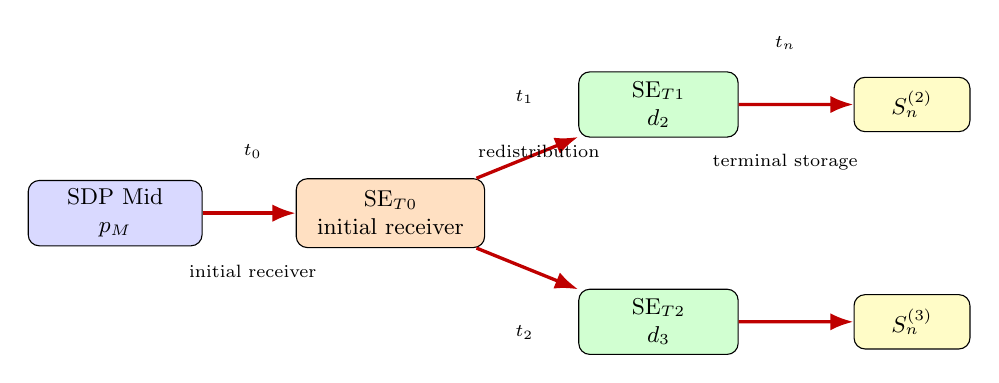
\begin{tikzpicture}[
>=Latex,
font=\small,
scale=0.92,
transform shape,
node distance=1.7cm and 1.8cm,
sdp/.style={draw, rounded corners, fill=blue!15, minimum width=2.4cm, minimum height=0.9cm, align=center},
sezero/.style={draw, rounded corners, fill=orange!24, minimum width=2.6cm, minimum height=0.95cm, align=center},
senonzero/.style={draw, rounded corners, fill=green!18, minimum width=2.2cm, minimum height=0.9cm, align=center},
sto/.style={draw, rounded corners, fill=yellow!22, minimum width=1.6cm, minimum height=0.75cm, align=center}
]

\node[sdp] (pm) at (0,0) {SDP Mid\\$p_M$};
\node[sezero] (se0) at (3.8,0) {\(\mathrm{SE}_{T0}\)\\initial receiver};
\node[senonzero] (d2) at (7.5,1.5) {\(\mathrm{SE}_{T1}\)\\$d_2$};
\node[senonzero] (d3) at (7.5,-1.5) {\(\mathrm{SE}_{T2}\)\\$d_3$};
\node[sto] (s2) at (11.0,1.5) {$S_n^{(2)}$};
\node[sto] (s3) at (11.0,-1.5) {$S_n^{(3)}$};

\draw[->, very thick, red!75!black] (pm) -- (se0);
\draw[->, very thick, red!75!black] (se0) -- (d2);
\draw[->, very thick, red!75!black] (se0) -- (d3);
\draw[->, very thick, red!75!black] (d2) -- (s2);
\draw[->, very thick, red!75!black] (d3) -- (s3);

\node[font=\scriptsize] at ($(pm)!0.5!(se0)+(0,0.85)$) {$t_0$};
\node[font=\scriptsize] at ($(se0)!0.5!(d2)+(0.0,0.85)$) {$t_1$};
\node[font=\scriptsize] at ($(se0)!0.5!(d3)+(0.0,-0.9)$) {$t_2$};
\node[font=\scriptsize] at ($(d2)!0.5!(s2)+(0,0.85)$) {$t_n$};

\node[font=\scriptsize] at ($(pm)!0.5!(se0)+(0,-0.8)$) {initial receiver};
\node[font=\scriptsize] at ($(se0)!0.5!(d2)+(0.2,0.1)$) {redistribution};
\node[font=\scriptsize] at ($(d2)!0.5!(s2)+(0,-0.8)$) {terminal storage};
\end{tikzpicture}
\caption{Simplified instantiation of the graph for a flow originating at a \emph{Mid} SDP. At \(t_0\), the data object is received by an \(\mathrm{SE}_{T0}\); at \(t_1\) and \(t_3\) (\textcolor{blue}{\(t_2\)?}), it is redistributed to \(\mathrm{SE}_{T1}\) and \(\mathrm{SE}_{T2}\), respectively; and at \(t_n\), it reaches the associated terminal nodes \(S_n\).}
\label{fig:arquitectura-red}
\end{figure}


\subsection{Sets and Indices}

Sets and indices are not merely notational devices: they define the geometry of the problem, the functional hierarchy of the network, and the level at which decisions are made.

\begin{description} 

\item[\(\V\)] The set of all nodes, \(\V = \Pset \cup \Iset \cup \Dset \cup \Sset \cup \Rset\), \textcolor{red}{where the subsets \(\Pset\), \(\Iset\), \(\Dset\),\(\Sset\), and \(\Rset\) each serve distinct roles within the graph, as defined above}. It defines the support of the graph and is required because every flow, capacity, or activation equation must be formulated over a common universe of nodes. 

\item[\(\A\)] The set of directed arcs, \(\A \subseteq \V\times\V\). It is used to model links that are available in a specific direction and is required because latency, capacity, and availability may be asymmetric. 

\item[\(\Pset\)] The set of SDPs, \(\Pset = \PL \cup \PM\), with \(\|\PL|=|\PM|=1\). It serves to identify the physical origins of the data and is required because the first stage of the flow always begins at a source node belonging to this set. 

\item[\(\PL\)] The subset of SDPs of class \emph{Low}. It serves to distinguish the origin associated with the low spectral range and is required because the provenance of the data constrains connectivity, volume, and compatibility with initial reception. 

\item[\(\PM\)] The subset of SDPs of class \emph{Mid}. It serves to distinguish the medium spectral family and is required for the same structural reason as \(\PL\). 

\item[\(\Iset\)] The set of \emph{Storage Elements} of type \(T0\). It is used to determine the point in the network at which each data object is initially received and is required because \(\mathrm{SE}_{T0}\) constitutes the primary interface between the SDP environment and the distributed SRC network. 

\item[\(\Dset\)] The set of \emph{Storage Elements} of types \(T1, T2, \dots\). It is used to model nodes specialised in redistribution, transfer services, and connection to final storage; it is required because the real architecture separates initial reception from subsequent transport and persistence layers.

\item[\(\Eset\)] The set of \emph{Storage Elements} that may act as initial receivers, \(\Eset=\Iset\cup\Dset\). It serves to unify \(\mathrm{SE}_{T0}\) and non-\(T0\) \emph{Storage Elements} that may receive data directly from an SDP, and is required because some \(T1, T2, \dots\) nodes admit direct input when the data size lies below their reception thresholds. 

\item[\(\Sset\)] The set of storage nodes. It is used to represent the persistent destinations of the replicas and is required because the final decision concerns not only transporting the data, but also determining where it is ultimately stored. 

\item[\(\Rset\)] The set of intermediate transit nodes. It is used to enable multi-hop routing without forcing every transmission to be direct and is required because, in global networks, the optimal path rarely coincides with a single hop between origin and destination. 

\item[\(\Cset\)] The finite set of \emph{SKA Regional Centres} (SRCs). It serves to introduce centre-level diversity, operational affinity, and replica-dispersion policies, and is required because the SRC network is distributed across multiple regional centres. 

\item[\(\Kset\)] The set of data objects or discretised demands. It is used to treat each scientific product as a distinct commodity and is required because volume, number of replicas, and optimal route may vary from one object to another. 

\item[\(\Mset\)] The set of potential replica positions, \(\Mset = \{1,\dots,|\Sset|\}\). It is used to index the first, second, third, and subsequent replicas, and is required because the number of copies is not fixed but is instead a model decision. 

\item[\(\Apre\)] The subset of arcs admissible in the SDP \(\to\) initial reception stage, \(\Apost\subseteq\A\). It is used to impose the logical ordering of the first stage and is required to exclude physically incompatible routes. 

\item[\(\Apost\)] The subset of arcs admissible in the stage following initial reception, \(\Apre\subseteq\A\). It is used to model redistribution from the receiving node towards other services and storage, and is required because the second stage has an operational semantics distinct from that of the first. 

\end{description}


The index \(v\) ranges over generic nodes, \(a\) over arcs, \(k\) over data objects, \(r\) over replica positions, \(i\) over \(\mathrm{SE}_{T0}\), \(d\) over non-\(T0\) \emph{Storage Elements}, \(s\) over storage nodes, and \(c\) over SRCs. 

Each node \(v\in\V\) belongs to an SRC \(\kappa(v)\in\Cset\). In addition, each storage node \(s\in\Sset\) has a parent non-\(T0\) \emph{Storage Element} \(\rho(s)\in\Dset\), so that \(\Gamma(d)=\{s\in\Sset: \rho(s)=d\}\) for all \(d\in\Dset\). For each SRC \(c\in\Cset\), we also define \(\Sset_c=\{s\in\Sset:\kappa(s)=c\}\).

The mapping \(\kappa(v)\) identifies the SRC to which node \(v\) belongs and is used to impose centre-level diversity and regional operational constraints. The mapping \(\rho(s)\) associates each storage node with its parent \emph{Storage Element} and is used to represent the last mile of the architecture. The set \(\Gamma(d)\) collects the storage nodes associated with the non-\(T0\) \emph{Storage Element} (d) and serves to link each transfer service to its local infrastructure. Similarly, \(\Sset_c\) gathers the storage nodes located in SRC (c) and is used when it is necessary to limit the concentration of replicas within a single centre.


Consistently with the physical architecture, every arc entering a storage node originates from its parent non-\(T0\) \emph{Storage Element}; that is,

\begin{equation}
\nonumber \delta^{-}(s)=\{(\rho(s),s)\},
\qquad \forall s\in\Sset,
\end{equation}

where \(\delta^{+}(v)\) and \(\delta^{-}(v)\) denote the sets of outgoing and incoming arcs of node \(v\in\V\), respectively. These sets are used to formulate the flow conservation equations and are required because the model must distinguish explicitly between the traffic entering and leaving each node.



\subsection{Parameters}


Each parameter specifies a physical, economic, or operational property of the system; accordingly, it is useful to state clearly what it represents, what role it plays, and why it appears in the model.

\begin{description} 

\item[\(o_k\)] Identifies the SDP from which data object \(k\) originates, with \(o_k\in\Pset\). It is used to fix the source node in the first flow conservation constraint and is required because each product arises physically at a single SDP. 

\item[\(q_k\)] The volume of data object \(k\), with \(q_k>0\). It is used to scale costs, times, energy consumption, occupancy, and capacity, and is required because transferring one petabyte does not have the same effect as transferring a few terabytes. 

\item[\(b_{kv}\)] The compatibility parameter between data object \(k\) and the initial receiving \emph{Storage Element} \(v\in\Eset\), with \(b_{kv}\in\{0,1\}\). It is used to reflect technical, policy, spectral, and type-based compatibility \(T0/T1/T2/\dots\), and is required because not all nodes can receive every flow. 

\item[\(\tau_v\)] The type label of \emph{Storage Element} \(v\in\Eset\), with \(\tau_v\in\{T0,T1,T2,\dots\}\). It is used to distinguish \(\mathrm{SE}_{T0}\) from subsequent \emph{Storage Elements} and is required because the two families do not provide exactly the same services. 

\item[\(\mu_v\)] Indicates whether \emph{Storage Element} \(v\in\Eset\) is \emph{Major} or \emph{Minor}, with \(\mu_v\in\{\mathrm{Major},\mathrm{Minor}\}\). It is used to distinguish capacity profiles and direct-reception capability and is required because the architecture does not treat all operational nodes identically. 

\item[\(Q_v^{\mathrm{dir}}\)] The maximum size of data object that \emph{Storage Element} \(v\in\Eset\) may receive directly from an SDP, with \(Q_v^{\mathrm{dir}}>0\). It is used to prevent an SDP from sending excessively large objects to nodes not designed to receive them, and is required because some non-\(T0\) \emph{Storage Elements} can only accept small or medium-sized data. 

\item[\(\omega_a\)] Indicates whether the transfer service associated with link \(a\in\A\) is operationally available, with \(\omega_a\in\{0,1\}\). It is used to deactivate links whose endpoint services are not ready to send or receive transfers and is required because actual availability depends on service activation, not solely on the physical circuit. 

\item[\(U_a\)] The bandwidth capacity of link \(a\in\A\), with \(U_a>0\). It is used to limit aggregate flow and is required because every physical link has finite bandwidth. 

\item[\(\ell_a\)] The propagation latency of link \(a\in\A\), with \(\ell_a\ge 0\). It is used to quantify delay and is required because geographical distance and network technology affect transit time. 

\item[\(t_a\)] The effective transmission time per unit of flow on link \(a\in\A\), with \(t_a\ge 0\). It is used to represent the pure temporal cost of transport and is required because total delay is not determined solely by propagation: serialisation and protocol time must also be considered. 

\item[\(\varphi_a\)] The failure rate of link \(a\in\A\), with \(\varphi_a\in[0,1]\). It is used to penalise fragile routes and is required because the reliability of a path is as important as its speed. 

\item[\(d_a\)] The geographical distance associated with link  \(a\in\A\), with \(d_a\ge 0\). It is used to approximate re-routing effects, geographical exposure, and the cost of long routes, and is required because physical length influences both operation and resilience. 

\item[\(\gamma_a\)] The congestion penalty coefficient of link \(a\in\A\), with \(\gamma_a>0\). It is used to weight the relative importance of queueing on each link and is required because not all congestion has the same operational impact. 

\item[\(\hat c_a\)] The fixed deployment or activation cost of link \(a\in\A\), with \(\hat c_a\ge 0\). It is used to model CAPEX or fixed usage cost and is required because maintaining a circuit or service in an available state entails a baseline cost. 

\item[\(c_a\)] The variable economic transfer cost on link \(a\in\A\), with \(c_a\ge 0\). It is used to monetise the traffic actually carried and is required because transporting large volumes consumes billable resources. 

\item[\(e_a\)] The energy consumption per unit of flow on link \(a\in\A\), with \(e_a\ge 0\). It is used to measure the energy footprint of transmission and is required because moving data at global scale entails a significant energy cost. 

\item[\(\hat c_v\)] The fixed deployment or equipment cost of node \(v\in\Iset\cup\Dset\cup\Sset\), with \(\hat c_v\ge 0\). It is used to represent infrastructure investment and is required because activating \(\mathrm{SE}_{T0}\), non-\(T0\) \emph{Storage Elements}, or storage resources is not cost-free. 

\item[\(c_v^{\mathrm{proc}}\)] The economic processing cost per unit of data at node \(v\in\Iset\cup\Dset\cup\Sset\), with \(c_v^{\mathrm{proc}}\ge 0\). It is used to monetise initial reception, routing, or disk-writing tasks and is required because local data handling consumes computational resources. 

\item[\(e_v^{\mathrm{proc}}\)] The processing energy consumption per unit of data at node \(v\in\Iset\cup\Dset\cup\Sset\), with \(e_v^{\mathrm{proc}}\ge 0\). It is used to quantify the internal energy cost of the node and is required because energy is consumed both on the links and in local computation. 

\item[\(t_v^{\mathrm{proc}}\)] The processing time per unit of data at node \(v\in\Iset\cup\Dset\cup\Sset\), with \(t_v^{\mathrm{proc}}\ge 0\). It is used to model delay due to initial reception, handling, or writing and is required because the bottleneck may lie at the node rather than solely on the link. 

\item[\(H_v\)] The processing capacity of node \(v\in\Iset\cup\Dset\cup\Sset\), with \(H_v>0\). It is used to prevent overload of CPU, I/O, or internal services and is required because nodal infrastructure has a maximum throughput. 

\item[\(M_v\)]  The temporary space or \emph{buffer} capacity of node \(v\in\Iset\cup\Dset\cup\Sset\), with \(M_v>0\). It is used to verify that the data fit during transfer or processing and is required because a node may have sufficient compute capacity but insufficient transient space. 

\item[\(B_s\)] The persistent capacity of storage node \(s\in\Sset\), with \(B_s>0\). It is used to ensure that the replica can be permanently accommodated and is required because the ultimate aim of the problem is to preserve the data in stable storage. 

\item[\(Q^{\mathrm{large}}\)] The size threshold for classifying an object as large, with \(Q^{\mathrm{large}}>0\). It is used to adapt the replication policy to the data volume and is required because very large objects may render extensive replication infeasible. 

\item[\(\overline\Phi_k\)] The maximum failure-exposure budget for data object \(k\), with \(\overline\Phi_k\ge 0\). It is used to limit excessively fragile routes and is required whenever a maximum acceptable level of risk is imposed. 

\item[\(D_{ss'}\)] The geographical distance between two storage nodes \(s,s'\in\Sset\), with \(D_{ss'}\ge 0\). It is used to measure geographical dispersion between replicas and is required because resilience to regional incidents demands spatial separation. 

\item[\(\Delta_k^{\min}\)] The minimum separation required between two replicas of data object \(k\), with \(\Delta_k^{\min}\ge 0\). It is used to translate the resilience policy into a mathematical constraint and is required to prevent two copies from being placed excessively close to one another. 

\item[\(\pi_E\)] The unit price of energy, with \(\pi_E\ge 0\). It is used to convert physical consumption into operational economic cost and is required because sustainability and cost are not necessarily the same quantity. 

\item[\(\overline\eta\)] The maximum permitted utilisation of links, with \(\overline\eta\in(0,1)\). It is used to maintain queue stability and is required because operating close to one hundred per cent utilisation leads to explosive delays. 

\item[\(\lambda_C,\lambda_E,\lambda_T,\lambda_G,\lambda_{RR},\lambda_{\eta}\)] The non-negative weights of the multi-objective function. They are used to prioritise economic cost, energy, time, congestion, re-routing, and load balancing, and are required because the real problem involves several simultaneous criteria. 

\end{description}


The minimum number of replicas depends on the size of the data object and is determined by

\begin{equation}
\underline R_k=
\begin{cases}
1, & q_k > Q^{\mathrm{large}},\\
2, & q_k \le Q^{\mathrm{large}},
\end{cases}
\qquad \forall k\in\Kset.
\end{equation}


In particular, local links between non-\(T0\) \emph{Storage Elements} and storage nodes may be modelled with capacities \(U_a\in{10,25,100}\) Gbps when they represent local Ethernet, whereas intercontinental and backbone links inherit their parameters from the WAN or Internet infrastructure on which they rely.


\begin{comment}
\begin{itemize}
    \item $Size_{d} \in \mathbb{R}^+$ denotes the size of data item $d \in D$.
    \item \textcolor{blue}{${Size_{sof}} \in \mathbb{R}^+$ denotes the processing requirements (e.g., software) associated with node $s \in S$} 
    \item $f_{k,n,s}$ denotes the flow of data item $d \in D$ from node $n \in N$ to storage node $s \in S$.
\end{itemize}
\end{comment}


\subsection{Decision variables}

The decision variables specify which infrastructure is activated, where each data object enters the system, and how its replicas are distributed across the network.

\begin{description}

\item[\(x_v\)] A binary variable equal to \(1\) if node \(v\in\Iset\cup\Dset\cup\Sset\) is activated. It is used to determine which infrastructure is brought into service and is required because activating nodes entails fixed costs and capacity implications. 

\item[\(y_a\)] A binary variable equal to \(1\) if link \(a\in\A\) is activated or used. It is used to design the operational logical network for the time instant under consideration and is required because not all available links need necessarily be utilised. 

\item[\(\alpha_{kv}\)] A binary variable equal to \(1\) if data object \(k\) is initially received at \emph{Storage Element} \(v\in\Eset\). It is used to determine the entry point into the SRC network and is required because the initial reception point influences latency, distance, and the subsequent distribution of replicas. 

\item[\(w_{kr}\)] A binary variable equal to \(1\) if potential replica \(r\in\Mset\) of data object \(k\) actually exists. It is used to convert the number of replicas into a binary decision and is required because redundancy is one of the central elements of the problem. 

\item[\(\beta_{krv}\)] A binary variable equal to \(1\) if replica \(r\) of data object \(k\) departs from the initial receiving \emph{Storage Element} \(v\in\Eset\). It is used to link the initial reception decision with the replication stage and is required to prevent a replica from departing from a node other than the one that initially received the data. 

\item[\(z_{krs}\)] A binary variable equal to \(1\) if replica \(r\) of data object \(k\) is ultimately stored at \(s\in\Sset\). It is used to assign specific persistent destinations and is required because the replication policy must be translated into physical storage nodes. 

\item[\(f_a^{0k}\)] The flow of data object \(k\) over link (\(a\in\A\) during the SDP \(\to\) initial reception stage. It is used to model transport from the SDP to the initial receiving node and is required because the first stage has specific constraints and costs. 

\item[\(f_a^{1kr}\)] The flow of replica \(r\) of data object \(k\) over link \(a\in\A\) during the stage following initial reception. It is used to model each distributed copy and is required because each replica may follow a different route. 

\item[\(g_i,g_d,g_s\)] The loads processed by \(\mathrm{SE}_{T0}\), non-\(T0\) \emph{Storage Elements}, and storage nodes, respectively. They are used to link flows with processing costs and limits and are required because a node does not merely transport data: it also receives, processes, classifies, or writes it. 

\item[\(\eta\)] The maximum relative utilisation of the links, with \(\eta\in[0,\overline\eta]\). It serves as an auxiliary load-balancing variable and is required to prevent solutions that saturate a small number of links even when the average cost appears low.

\end{description}

By convention, \(f_a^{0k}=0\) if \(a\notin\Apre\), and \(f_a^{1kr}=0\) if \(a\notin\Apost\). This convention imposes the logical ordering SDP \(\to\) initial reception \(\to\) non-\(T0\) \emph{Storage Element} \(\to\) storage, without excluding multi-hop routes.



\subsection{Cost Components and Objective Function}

The total flow traversing a physical link is given by

\begin{equation}
F_a = \sum_{k\in\Kset} f_a^{0k} + \sum_{k\in\Kset}\sum_{r\in\Mset} f_a^{1kr},
\qquad \forall a\in\A.
\end{equation}

The processing loads associated with each family of nodes are given by


\begin{align}
g_i &= \sum_{k\in\Kset} q_k\,\alpha_{ki}
      + \sum_{k\in\Kset}\sum_{r\in\Mset} q_k\,\beta_{kri},
       &&\forall i\in\Iset,\\[1ex]
\begin{split}
g_d &= \sum_{k\in\Kset} q_k\,\alpha_{kd}
      + \sum_{k\in\Kset}\sum_{r\in\Mset} q_k\,\beta_{krd} \\
    &\quad + \sum_{k\in\Kset}\sum_{r\in\Mset}\sum_{s\in\Gamma(d)} q_k\,z_{krs},
\end{split}
       && \forall d\in\Dset,\\[1ex]
g_s &= \sum_{k\in\Kset}\sum_{r\in\Mset} q_k\,z_{krs},
       &&\forall s\in\Sset.
\end{align}


The infrastructure cost (CAPEX) is given by

\begin{equation}
C^{\mathrm{capex}}
= \sum_{a\in\A} \hat c_a\,y_a
+ \sum_{v\in\Iset\cup\Dset\cup\Sset} \hat c_v\,x_v.
\end{equation}

The direct economic cost of transfer and processing is given by

\begin{align}
\begin{split}
C^{\mathrm{tr}}
&= \sum_{a\in\A} c_a\,F_a
+ \sum_{i\in\Iset} c_i^{\mathrm{proc}}\,g_i \\
&\quad + \sum_{d\in\Dset} c_d^{\mathrm{proc}}\,g_d
+ \sum_{s\in\Sset} c_s^{\mathrm{proc}}\,g_s.
\end{split}
\end{align}


The total physical energy consumption is given by

\begin{align}
\begin{split}
E
&= \sum_{a\in\A} e_a\,F_a
+ \sum_{i\in\Iset} e_i^{\mathrm{proc}}\,g_i \\
&\quad + \sum_{d\in\Dset} e_d^{\mathrm{proc}}\,g_d
+ \sum_{s\in\Sset} e_s^{\mathrm{proc}}\,g_s
\end{split}
\end{align}

The energy operating cost (OPEX) is modelled as


\begin{equation}
C^{\mathrm{opex}} = \pi_E\,E
\end{equation}

Therefore, the total economic cost is given by

\begin{equation}
\label{ref:econ}
C_{\mathrm{econ}} = C^{\mathrm{capex}} + C^{\mathrm{tr}} + C^{\mathrm{opex}}.
\end{equation}

The total temporal cost, comprising propagation latency, transmission time, and processing time, is expressed as

\begin{align}
\begin{split}
T
&= \sum_{a\in\A} (\ell_a+t_a)\,F_a
+ \sum_{i\in\Iset} t_i^{\mathrm{proc}}\,g_i \\
&\quad + \sum_{d\in\Dset} t_d^{\mathrm{proc}}\,g_d
+ \sum_{s\in\Sset} t_s^{\mathrm{proc}}\,g_s.
\end{split}
\end{align}


To model queueing congestion, the following convex function is adopted:

\begin{equation}
\Psi_a(F_a)=\frac{F_a}{U_a-F_a},
\qquad 0\le F_a < U_a,
\qquad \forall a\in\A,
\end{equation}

which is strictly increasing and convex over its domain, since

\begin{equation}
\Psi_a''(F_a)=\frac{2U_a}{(U_a-F_a)^3}>0,
\qquad \forall a\in\A.
\end{equation}

The aggregate congestion cost is therefore given by

\begin{equation}
C_{\mathrm{cong}} = \sum_{a\in\A} \gamma_a\,\Psi_a(F_a).
\end{equation}

The re-routing cost is approximated by the expected exposure to failure, weighted by the distance of the link,

\begin{equation}
C_{\mathrm{RR}} = \sum_{a\in\A} d_a\,\varphi_a\,F_a.
\end{equation}


This yields a multi-objective optimisation problem:

\begin{equation}
\min \; \lambda_C C_{\mathrm{econ}}
+ \lambda_E E
+ \lambda_T T
+ \lambda_G C_{\mathrm{cong}}
+ \lambda_{RR} C_{\mathrm{RR}}
+ \lambda_{\eta}\,\eta
\end{equation}


The presence of \(\eta\) penalises configurations with high peak utilisation and serves as an explicit load-balancing criterion. Where hierarchical prioritisation is desired, a lexicographic formulation or an \(\varepsilon\)-constraint method may be employed.


\subsubsection*{Interpretation of the Cost Components and the Objective Function}


\begin{description}

\item[\(F_a\)] The total flow traversing link \(a\). It is used to aggregate, into a single quantity, the traffic of the SDP \(\to\) initial reception stage and the traffic associated with all replicas. It is required because the capacity, congestion, energy consumption, and cost of the link depend on total utilisation rather than on an isolated commodity alone. 

\item[\(g_i,g_d,g_s\)] The nodal processing loads. They are used to measure the amount of actual work performed by each node and are required because nodal costs and processing times depend on the load handled. 

\item[\(C^{\mathrm{capex}}\)] The fixed infrastructure cost. It is used to penalise the activation or deployment of nodes and links and is required because a highly dispersed architecture may be fast, but excessively expensive to keep installed. 

\item[\(C^{\mathrm{tr}}\)] The direct economic cost of transport and processing. It is used to monetise the effective use of the network and nodes and is required because each unit of traffic has a marginal cost. 

\item[\(E\)] The total physical energy consumption. It is used to measure the energy footprint and is required because sustainability and electricity demand are relevant criteria in their own right. 

\item[\(C^{\mathrm{opex}}\)] The operating cost associated with energy. It is used to translate energy consumption into monetary expenditure and is required because the same solution may be inexpensive in CAPEX terms but costly in day-to-day operation. 

\item[\(C_{\mathrm{econ}}\)] The total economic cost. It is used to integrate deployment, transfer, processing, and energy into a single monetary quantity and is required because the final decision is often constrained by overall budgets. 

\item[\(T\)] The total temporal cost. It is used to quantify the aggregate transit and processing time and is required because the scientific objective may demand rapid data availability. 

\item[\(\Psi_a(F_a)\)] The convex congestion function of link (a). It is used to capture the fact that queueing delay increases non-linearly as the link approaches saturation and is required because a linear penalty does not adequately reflect the actual behaviour of queues. 

\item[\(C_{\mathrm{cong}}\)] The aggregate congestion cost. It is used to discourage excessive use of heavily loaded links and is required in order to obtain more stable and robust solutions. 

\item[\(C_{\mathrm{RR}}\)] The re-routing cost. It is used to penalise long and fragile paths, where a failure would necessitate costly route recomposition, and is required because operational resilience does not depend solely on the nominal state of the network. 

\item[\(\eta\)] In the objective function, this acts as a peak-utilisation penalty. It is used to promote load balancing across links and is required because a well-balanced network is generally more robust and more predictable. 

\item[\(\lambda_C,\lambda_E,\lambda_T,\lambda_G,\lambda_{RR},\lambda_{\eta}\)] These determine the relative importance of each criterion. They are used to adapt the model to scientific, economic, or environmental priorities and are required because the optimal solution varies according to the decision context. The weights associated with each criterion may be defined at this point.

\end{description}


The objective function is required because the real problem does not pursue a single goal. Minimising monetary cost alone would tend to concentrate flows and reduce redundancy; minimising time alone could lead to the activation of an excessive number of resources; and minimising energy alone might force the use of slow routes. A multi-objective formulation makes it possible to balance these competing interests in a controlled manner.



\subsection{Constraints}

\subsection*{Assignment of Initial Reception and Replicas}

At least one active \(\mathrm{SE}_{T0}\) must always be available:

\begin{equation}
\sum_{i\in\Iset} x_i \ge 1.
\end{equation}

Each data object must be initially received by a unique compatible and activated \emph{Storage Element}:


\begin{align}
&\sum_{v\in\Eset} \alpha_{kv} = 1,
&& \forall k\in\Kset,\\[1ex]
&\left.
\begin{aligned}
\alpha_{kv} &\le b_{kv} \\
\alpha_{kv} &\le x_v \\
q_k\,\alpha_{kv} &\le Q_v^{\mathrm{dir}}\,x_v 
\end{aligned}
\right\}
&& \forall k\in\Kset,\, v\in\Eset.
\end{align}



The final inequality allows certain non-\(T0\) \emph{Storage Elements} to receive data directly from an SDP only when the size of the object lies below their operational threshold; this threshold also encapsulates the distinction between \emph{Major} and \emph{Minor} nodes.

The number of active replicas is bounded below by the size-dependent policy:

\begin{equation}
\underline R_k \le \sum_{r\in\Mset} w_{kr},
\qquad \forall k\in\Kset.
\end{equation}

Each active replica is assigned to a unique storage node:

\begin{align}
&\sum_{s\in\Sset} z_{krs} = w_{kr},
&& \forall k\in\Kset,\, r\in\Mset,\\[1ex]
&\left.
\begin{aligned}
z_{krs} &\le x_s \\
z_{krs} &\le x_{\rho(s)}
\end{aligned}
\right\}
&& \forall k\in\Kset,\, r\in\Mset,\, s\in\Sset
\end{align}


To ensure structural resilience, a given data object may not use the same non-\(T0\) \emph{Storage Element} more than once:

\begin{equation}
\sum_{r\in\Mset}\sum_{s\in\Gamma(d)} z_{krs} \le 1,
\qquad \forall k\in\Kset,\ \forall d\in\Dset.
\end{equation}


If diversity across SRCs is required between replicas, the following additional constraint may be imposed:

\begin{equation}
\sum_{r\in\Mset}\sum_{s\in\Sset_c} z_{krs} \le 1,
\qquad \forall k\in\Kset,\ \forall c\in\Cset.
\end{equation}

The minimum geographical dispersion between replicas is modelled by

\begin{equation}
\begin{split}
z_{krs} + z_{kr's'} &\le 1, \\
&\forall k\in\Kset,\ \forall r\neq r'\in\Mset, \\
&\forall (s,s')\in\Sset\times\Sset : D_{ss'}<\Delta_k^{\min}
\end{split}
\end{equation}

\subsection*{Linearisation of the origin of each replica}

Replica \(r\) of data object \(k\) departs from the same initial receiving \emph{Storage Element} selected for that data object. The corresponding binary linearisation is

\begin{comment}
\begin{align}
\beta_{krv} &\le \alpha_{kv},
&& \forall k\in\Kset,\ \forall r\in\Mset,\ \forall v\in\Eset,\\
\beta_{krv} &\le w_{kr},
&& \forall k\in\Kset,\ \forall r\in\Mset,\ \forall v\in\Eset,\\
\beta_{krv} &\ge \alpha_{kv}+w_{kr}-1,
&& \forall k\in\Kset,\ \forall r\in\Mset,\ \forall v\in\Eset,\\
\sum_{v\in\Eset} \beta_{krv} &= w_{kr},
&& \forall k\in\Kset,\ \forall r\in\Mset.
\end{align}
\end{comment}


\begin{align}
&\left.
\begin{aligned}
\beta_{krv} &\le \alpha_{kv} \\
\beta_{krv} &\le w_{kr} \\
\beta_{krv} &\ge \alpha_{kv}+w_{kr}-1 
\end{aligned}
\right\}
&& \forall k\in\Kset, r\in\Mset, v\in\Eset,\\[1.5ex]
&\sum_{v\in\Eset} \beta_{krv} = w_{kr},
&& \forall k\in\Kset, r\in\Mset.
\end{align}


\subsection*{Flow Conservation}

The stage preceding redistribution transfers exactly one copy of the data object from its source SDP to the selected initial receiving \emph{Storage Element}:

\begin{equation}
\begin{split}
\sum_{a\in\delta^{+}(v)} f_a^{0k} &- \sum_{a\in\delta^{-}(v)} f_a^{0k} = \\
&\begin{cases}
q_k, & v = o_k,\\
-q_k\,\alpha_{kv}, & v\in\Eset,\\
0, & v\in\V\setminus(\{o_k\}\cup\Eset),
\end{cases} \\[1.5ex]
&\forall k\in\Kset,\, v\in\V.
\end{split}
\end{equation}

The stage following initial reception generates one complete copy for each active replica:

\begin{equation}
\begin{split}
\sum_{a\in\delta^{+}(v)} f_a^{1kr} &- \sum_{a\in\delta^{-}(v)} f_a^{1kr} = \\
&\begin{cases}
q_k\,\beta_{krv}, & v\in\Eset,\\
-q_k\,z_{krv}, & v\in\Sset,\\
0, & v\in\V\setminus(\Eset\cup\Sset),
\end{cases} \\[1.5ex]
&\forall k\in\Kset,\, r\in\Mset,\, v\in\V.
\end{split}
\end{equation}

These equations ensure that, except at the source and destination, no intermediate node creates or destroys flow, and they naturally allow for routes comprising one or more hops.

\paragraph{SDP-to-initial-reception stage.} The first flow conservation equation imposes that each data object \(k\) is transmitted exactly once from its source \(o_k\) with total flow \(q_k\). That same volume must be absorbed exactly at the initial receiving node selected through \(\alpha_{kv}\). All intermediate nodes have zero net balance. This stage serves to ensure that the initial transfer from Australia or South Africa to the SRC network faithfully reproduces a single copy of the data object and that no artificial branching arises prior to redistribution.


\paragraph{Redistribution and storage stage.} The second equation is applied on a replica-by-replica basis. For each \((k,r)\), the initial receiving \emph{Storage Element} that originates the copy injects a flow \(q_k\,\beta_{krv}\), while the selected storage node absorbs exactly \(q_k\,z_{krs}\). Once again, every intermediate node—whether a non-\(T0\) \emph{Storage Element} or a transit node—preserves flow with zero net balance. This stage serves to ensure that each active replica constitutes a complete copy of the data object rather than an incomplete fraction.

\paragraph{Joint interpretation of both stages.} Flow conservation is imposed at two levels because the physical process itself also unfolds in two stages: first, the raw or processed data are transported to an entry point within the SRC federation, and only thereafter are replication and distribution decisions made. Separating these two stages makes it possible to assign distinct costs, latencies, and constraints to each segment of the architecture, while respecting the operational logic of the system.


\paragraph{Why this is indispensable.} Without flow conservation, the model could produce solutions that are mathematically inexpensive yet physically impossible: data that disappear midway through the network, replicas that arise without having been transmitted, or destinations that receive less volume than required. Flow conservation ensures the material consistency of the problem at every stage.


\subsection*{Capacity, Availability, and Stability of the Links}

The physical capacity of the link and the operational availability of the associated transfer service are imposed through

\begin{align}
F_a &\le U_a\,y_a,
&& \forall a\in\A,\\
y_a &\le \omega_a,
&& \forall a\in\A.
\end{align}


The maximum relative utilisation is modelled by

\begin{equation}
F_a \le \eta\,U_a,
\qquad \forall a\in\A,
\end{equation}

subject to the stability bound

\begin{equation}
\nonumber 0\le \eta \le \overline\eta < 1.
\end{equation}

If a link is connected to a node whose service stack has not been activated to receive or transmit transfers, that link cannot be used. Defining

\begin{equation}
\bar x_v=
\begin{cases}
1, & v\in\Pset\cup\Rset,\\
x_v, & v\in\Iset\cup\Dset\cup\Sset,
\end{cases}
\qquad \forall v\in\V,
\end{equation}


the following consistency constraints are imposed


\begin{equation}
y_{(u,v)} \le \bar x_u,
\qquad
y_{(u,v)} \le \bar x_v,
\qquad \forall (u,v)\in\A.
\end{equation}


\subsection*{Processing and Storage Capacity of the Nodes}

The loads processed by \(\mathrm{SE}_{T0}\), non-\(T0\) \emph{Storage Elements}, and storage nodes must not exceed their installed capacities:

\begin{align}
g_i &\le H_i\,x_i,
&& \forall i\in\Iset,\\
g_d &\le H_d\,x_d,
&& \forall d\in\Dset,\\
g_s &\le H_s\,x_s,
&& \forall s\in\Sset.
\end{align}


The aggregate occupation of temporary storage space at the initial receiving nodes, non-\(T0\) \emph{Storage Elements}, and storage nodes must be feasible:


\begin{align}
&\sum_{k\in\Kset} q_k\,\alpha_{ki} \le M_i\,x_i,
\qquad \forall i\in\Iset,\\[2ex]
&\!\begin{aligned}
  &\sum_{k\in\Kset} q_k\,\alpha_{kd} 
   + \sum_{k\in\Kset}\sum_{r\in\Mset} q_k\,\beta_{krd} \\
  &\quad + \sum_{k\in\Kset}\sum_{r\in\Mset}\sum_{s\in\Gamma(d)} q_k\,z_{krs} \le M_d\,x_d, \\
  &\qquad\qquad \forall d\in\Dset,
\end{aligned}\\[2ex]
&\sum_{k\in\Kset}\sum_{r\in\Mset} q_k\,z_{krs} \le M_s\,x_s,
\qquad \forall s\in\Sset.
\end{align}


Moreover, each individual data object must fit within the node that processes or stores it:

\begin{alignat}{2}
&q_k\,\alpha_{ki} \le M_i\,x_i,
&& \forall k\in\Kset,\, i\in\Iset,\\[2ex]
&\!\begin{aligned}
  &q_k\,\alpha_{kd} + q_k\sum_{r\in\Mset} \beta_{krd} \\
  &\quad + q_k\sum_{r\in\Mset}\sum_{s\in\Gamma(d)} z_{krs} \le M_d\,x_d, \\
  &\qquad\qquad \forall k\in\Kset,\, d\in\Dset,
\end{aligned} && \\[2ex]
&\!\begin{aligned}
  &q_k\,z_{krs} \le M_s\,x_s, \\
  &\qquad\qquad \forall k\in\Kset,\, r\in\Mset,\, s\in\Sset.
\end{aligned} &&
\end{alignat}


The persistent storage capacity is expressed as

\begin{equation}
\sum_{k\in\Kset}\sum_{r\in\Mset} q_k\,z_{krs} \le B_s\,x_s,
\qquad \forall s\in\Sset,
\end{equation}


and, moreover, each individual replica must fit within the storage node that hosts it:

\begin{equation}
q_k\,z_{krs} \le B_s\,x_s,
\qquad \forall k\in\Kset,\ \forall r\in\Mset,\ \forall s\in\Sset
\end{equation}


\subsection*{Reliability and Exposure to Failure}


The cumulative exposure to links with high failure rates is controlled by

\begin{equation}
\sum_{a\in\A} \varphi_a\left(f_a^{0k} + \sum_{r\in\Mset} f_a^{1kr}\right)
\le \overline\Phi_k,
\qquad \forall k\in\Kset
\end{equation}


\begin{comment}
    
\subsection*{Domain of the Variables}

Finally,

\begin{align}
x_v &\in \{0,1\},
&& \forall v\in\Iset\cup\Dset\cup\Sset,\\
y_a &\in \{0,1\},
&& \forall a\in\A,\\
\alpha_{kv} &\in \{0,1\},
&& \forall k\in\Kset,\ \forall v\in\Eset,\\
w_{kr} &\in \{0,1\},
&& \forall k\in\Kset,\ \forall r\in\Mset,\\
\beta_{krv} &\in \{0,1\},
&& \forall k\in\Kset,\ \forall r\in\Mset,\ \forall v\in\Eset,\\
z_{krs} &\in \{0,1\},
&& \forall k\in\Kset,\ \forall r\in\Mset,\ \forall s\in\Sset,\\
f_a^{0k} &\ge 0,
&& \forall a\in\A,\ \forall k\in\Kset,\\
f_a^{1kr} &\ge 0,
&& \forall a\in\A,\ \forall k\in\Kset,\ \forall r\in\Mset,\\
g_i &\ge 0,
&& \forall i\in\Iset,\\
g_d &\ge 0,
&& \forall d\in\Dset,\\
g_s &\ge 0,
&& \forall s\in\Sset.
\end{align}

\end{comment}


\subsection{\textcolor{blue}{Problem Formalization}}


Based on the previous mathematical formulation, the multi-objective optimisation problem is formally defined as follows.


\begin{equation}
\begin{split}
\min \quad & \lambda_C C_{\mathrm{econ}} + \lambda_E E + \lambda_T T \\
& + \lambda_G C_{\mathrm{cong}} + \lambda_{RR} C_{\mathrm{RR}} + \lambda_{\eta} \eta
\end{split}
\end{equation}

\text{s.t.}
\begin{align}
& \sum_{i\in\Iset} x_i \ge 1, \\[2ex]
& \sum_{v\in\Eset} \alpha_{kv} = 1, && \forall k \in \Kset, \\[2ex]
& \underline R_k \le \sum_{r\in\Mset} w_{kr}, && \forall k \in \Kset, \\[2ex]
\begin{split}
  & \sum_{a\in\delta^{+}(v)} f_a^{0k} - \sum_{a\in\delta^{-}(v)} f_a^{0k} = \\
  &\quad \begin{cases}
    q_k, & v = o_k, \\
    -q_k \alpha_{kv}, & v \in \Eset, \\
    0, & v \in \V\setminus(\{o_k\} \cup \Eset),
  \end{cases} \\
  &\qquad\qquad \forall k \in \Kset, \, v \in \V,
\end{split} \\[2ex]
\begin{split}
  & \sum_{a\in\delta^{+}(v)} f_a^{1kr} - \sum_{a\in\delta^{-}(v)} f_a^{1kr} = \\
  &\quad \begin{cases}
    q_k \beta_{krv}, & v \in \Eset, \\
    -q_k z_{krs}, & v \in \Sset, \\
    0, & v \in \V\setminus(\Eset \cup \Sset),
  \end{cases} \\
  &\qquad\qquad \forall k \in \Kset, \, r \in \Mset, \, v \in \V,
\end{split} \\[2ex]
& F_a \le U_a y_a, && \forall a \in \A, \\[2ex]
& g_i \le H_i x_i, && \forall i \in \Iset, \\[2ex]
& g_d \le H_d x_d, && \forall d \in \Dset, \\[2ex]
& g_s \le H_s x_s, && \forall s \in \Sset, \\[2ex]
\begin{split}
  & \sum_{a\in\A} \varphi_a \left(f_a^{0k} + \sum_{r\in\Mset} f_a^{1kr}\right) \le \overline\Phi_k, \\
  &\qquad\qquad \forall k \in \Kset.
\end{split}
\end{align}


Where $x_v \in \{0,1\}, \forall v \in \Iset \cup \Dset \cup \Sset$ is a binary decision variable equal to 1 if node $v$ is activated and 0 otherwise. Similarly, $y_a \in \{0,1\}, \forall a \in \A$ is a binary decision variable equal to 1 if link $a$ is activated or utilized, and 0 otherwise. For each data object $k$ and storage element $v$, $\alpha_{kv} \in \{0,1\}, \forall k \in \Kset, \forall v \in \Eset$ is a binary parameter equal to 1 if object $k$ is initially received by storage element $v$, and 0 otherwise. For each object $k$ and replica index $r$, $w_{kr} \in \{0,1\}, \forall k \in \Kset, \forall r \in \Mset$ is a binary decision variable equal to 1 if replica $r$ of object $k$ is created, and 0 otherwise. Furthermore, $\beta_{krv} \in \{0,1\}, \forall k \in \Kset, \forall r \in \Mset, \forall v \in \Eset$ is a binary decision variable equal to 1 if replica $r$ of object $k$ is transmitted from storage element $v$, and 0 otherwise. For each object $k$, replica $r$, and node $s$,  $z_{krs} \in \{0,1\}, \forall k \in \Kset, \forall r \in \Mset, \forall s \in \Sset$ is a binary decision variable equal to 1 if replica $r$ of object $k$ is stored at node $s$, and 0 otherwise.

Flow variables are modelled as continuous non-negative variables. Specifically, $f_a^{0k} \ge 0, \forall a \in \A, \forall k \in \Kset$ denotes the quantity of object $k$ transmitted over link $a$ during the initial reception stage, whereas $f_a^{1kr} \ge 0, \forall a \in \A, \forall k \in \Kset, \forall r \in \Mset$ denotes the quantity of replica $r$ of object $k$ transmitted over link $a$ during the redistribution stage. In addition, the variables $g_i \ge 0, \forall i \in \Iset$, $g_d$, and $g_s$ are continuous variables representing processed load: $g_i$ denotes the load handled by $T_0$ storage elements, $g_d \ge 0, \forall d \in \Dset$ denotes the load handled by non-$T_0$ storage elements, and $g_s \ge 0,  \forall s \in \Sset$ denotes the load processed by storage nodes in general. Finally, $\eta$ is a continuous variable representing the maximum relative utilization across links, that is, the peak link utilization ratio.

Finally, in the multi-objective function, \(C_{\mathrm{econ}}\) \ref{ref:econ} denotes the total economic cost, including infrastructure, transfer, and operating costs; \(E\) represents the total physical energy consumption; \(T\) denotes the total temporal cost, including propagation and processing delays; \(C_{\mathrm{cong}}\) represents the aggregate congestion cost; \(C_{\mathrm{RR}}\) denotes the re-routing cost induced by failures; and \(\eta\) is an auxiliary variable introduced to promote load balancing among links.


\subsection{\textcolor{red}{Problem Complexity and Solution Approach}}

\section{Example of an Instantiation by SRC}
\label{Instantiation}

In this section, a small but complete instance of the model is specified in order to make the formulation immediately transparent to the reader. The instance represents a planning horizon of \(90\) days: Australia generates one \emph{Low} data object, South Africa generates two \emph{Med} data objects, and the SRC network must determine simultaneously the initial reception, the activation of links and nodes, the redistribution routes, and the final storage locations of the replicas.


\subsection{Representative Minimal but Complete Topology}

The instance comprises nine SRCs, each of which fulfils a distinct function within the network:

\begin{itemize} 
\item \(\mathrm{ausSRC}\): contains the \emph{Low} SDP \(p_L^{\mathrm{ausSRC}}\). 

\item \(\mathrm{zaSRC}\): contains the \emph{Mid} SDP \(p_M^{\mathrm{zaSRC}}\). 

\item \(\mathrm{espSRC}\): contains an initial receiver \(i_{\mathrm{espSRC}}^{T0}\), a redistribution \emph{Storage Element} \(d_{\mathrm{espSRC}}^{T1}\), and its two associated storage nodes. 

\item \(\mathrm{ukSRC}\): contains an initial receiver \(i_{\mathrm{ukSRC}}^{T0}\), a transit node \(r_{\mathrm{ukSRC}}\), a \emph{Storage Element} \(d_{\mathrm{ukSRC}}^{T1}\), and its two associated storage nodes. 

\item \(\mathrm{inSRC}\): contains the initial receiver \(i_{\mathrm{inSRC}}^{T0}\) and the transit node \(r_{\mathrm{inSRC}}\). 

\item \(\mathrm{deSRC}\): contains the backbone node \(r_{\mathrm{deSRC}}\), the \emph{Storage Element} \(d_{\mathrm{deSRC}}^{T2}\), and its two associated storage nodes. 

\item \(\mathrm{chSRC}\): contains the \emph{Storage Element} \(d_{\mathrm{chSRC}}^{T2}\) and its two associated storage nodes. 

\item \(\mathrm{caSRC}\): contains the \emph{Storage Element} \(d_{\mathrm{caSRC}}^{T2}\) and its two associated storage nodes. 

\item \(\mathrm{jpSRC}\): contains the \emph{Storage Element} \(d_{\mathrm{jpSRC}}^{T1}\) and its two associated storage nodes. 

\end{itemize}


\textcolor{blue}{Graph representation here...}

In the notation of the model, the sets are specified as follows:


\begin{align*}
\PL_{\mathrm{ej}} &= \{p_L^{\mathrm{ausSRC}}\}, \qquad
\PM_{\mathrm{ej}} = \{p_M^{\mathrm{zaSRC}}\}, \\[1ex]
\Pset_{\mathrm{ej}} &= \PL_{\mathrm{ej}} \cup \PM_{\mathrm{ej}}, \\[1.5ex]
\Cset_{\mathrm{ej}} &= \bigl\{\mathrm{ausSRC},\, \mathrm{zaSRC},\, \mathrm{espSRC},\, \mathrm{ukSRC},\, \mathrm{inSRC}, \\
&\quad \mathrm{chSRC},\, \mathrm{deSRC},\, \mathrm{caSRC},\, \mathrm{jpSRC}\bigr\}, \\[1.5ex]
\Iset_{\mathrm{ej}} &= \bigl\{i_{\mathrm{espSRC}}^{T0},\, i_{\mathrm{ukSRC}}^{T0},\, i_{\mathrm{inSRC}}^{T0}\bigr\}, \\[1.5ex]
\Dset_{\mathrm{ej}} &= \bigl\{d_{\mathrm{espSRC}}^{T1},\, d_{\mathrm{ukSRC}}^{T1},\, d_{\mathrm{deSRC}}^{T2}, \\
&\quad d_{\mathrm{chSRC}}^{T2},\, d_{\mathrm{caSRC}}^{T2},\, d_{\mathrm{jpSRC}}^{T1}\bigr\}, \\[1.5ex]
\Rset_{\mathrm{ej}} &= \{r_{\mathrm{ukSRC}},\, r_{\mathrm{deSRC}},\, r_{\mathrm{inSRC}}\}, \\[1ex]
\Eset_{\mathrm{ej}} &= \Iset_{\mathrm{ej}} \cup \Dset_{\mathrm{ej}}
\end{align*}


Each non-\(T0\) \emph{Storage Element} is associated with two terminal storage nodes:

\begin{align*}
\Gamma(d) &= \{s_{d,1},\, s_{d,2}\},
&& \forall d \in \Dset_{\mathrm{ej}}
\end{align*}

so that

\begin{align*}
\Sset_{\mathrm{ej}} &= \{s_{d,j}: d\in\Dset_{\mathrm{ej}},\, j=1,2\}, \quad
\Mset_{\mathrm{ej}} = \{1,\dots,12\}
\end{align*}

Furthermore,

\begin{align*}
\rho(s_{d,j}) &= d, \qquad \kappa(s_{d,j}) = \kappa(d), \\[1ex]
\kappa(v) &= \text{the SRC indicated by the subscript of } v.
\end{align*}

For example,
\begin{align*}
\Sset_{\mathrm{espSRC}} &= \Gamma(d_{\mathrm{espSRC}}^{T1}) \qquad
\Sset_{\mathrm{deSRC}} = \Gamma(d_{\mathrm{deSRC}}^{T2}).
\end{align*}


The topology is completed by defining two families of admissible arcs. The first, corresponding to the initial reception stage, permits either direct arrival or arrival via transit:

\begin{equation}
\nonumber
\begin{split}
\Apre_{\mathrm{ej}} \subseteq \bigl( \Pset_{\mathrm{ej}} &\times (\Iset_{\mathrm{ej}} \cup \{d_{\mathrm{ukSRC}}^{T1},\, d_{\mathrm{jpSRC}}^{T1}\}) \bigr) \\
&\cup (\Pset_{\mathrm{ej}} \times \Rset_{\mathrm{ej}}) \cup (\Rset_{\mathrm{ej}} \times \Eset_{\mathrm{ej}})
\end{split}
\end{equation}


The second, corresponding to subsequent redistribution, connects initial receiving nodes and backbone nodes, non-\(T0\) \emph{Storage Elements} and terminal storage:

\begin{equation}
\nonumber
\begin{split}
\Apost_{\mathrm{ej}} \subseteq \bigl( (\Iset_{\mathrm{ej}} &\cup \Dset_{\mathrm{ej}} \cup \Rset_{\mathrm{ej}}) \times (\Dset_{\mathrm{ej}} \cup \Rset_{\mathrm{ej}}) \bigr) \\
&\cup \bigl\{(d,s): d \in \Dset_{\mathrm{ej}},\, s \in \Gamma(d)\bigr\}.
\end{split}
\end{equation}

A representative subset of arcs is given by

\begin{align*}
& (p_L^{\mathrm{ausSRC}},i_{\mathrm{espSRC}}^{T0}),\,
  (p_L^{\mathrm{ausSRC}},i_{\mathrm{ukSRC}}^{T0}), \\
& (p_L^{\mathrm{ausSRC}},r_{\mathrm{inSRC}}),\,
  (p_M^{\mathrm{zaSRC}},r_{\mathrm{deSRC}}), \\
& (p_M^{\mathrm{zaSRC}},d_{\mathrm{ukSRC}}^{T1}),\,
  (r_{\mathrm{deSRC}},i_{\mathrm{espSRC}}^{T0}), \\
& (r_{\mathrm{deSRC}},d_{\mathrm{jpSRC}}^{T1}) \in \Apre_{\mathrm{ej}}, \\[1.5ex]
& (i_{\mathrm{espSRC}}^{T0},d_{\mathrm{espSRC}}^{T1}),\,
  (i_{\mathrm{espSRC}}^{T0},r_{\mathrm{deSRC}}), \\
& (r_{\mathrm{deSRC}},d_{\mathrm{deSRC}}^{T2}),\,
  (d_{\mathrm{ukSRC}}^{T1},r_{\mathrm{ukSRC}}), \\
& (r_{\mathrm{ukSRC}},d_{\mathrm{caSRC}}^{T2}),\,
  (d_{\mathrm{espSRC}}^{T1},s_{d_{\mathrm{espSRC}}^{T1},1}), \\
& (d_{\mathrm{caSRC}}^{T2},s_{d_{\mathrm{caSRC}}^{T2},1}) \in \Apost_{\mathrm{ej}}.
\end{align*}


\subsection{Demands, Compatibilities, and Resilience Rules}

Three data objects are considered:

\begin{align*}
&o_{k_1}=p_L^{\mathrm{ausSRC}}, && q_{k_1}=30\ \text{PB},\\
&o_{k_2}=p_M^{\mathrm{zaSRC}}, && q_{k_2}=12\ \text{PB},\\
&o_{k_3}=p_M^{\mathrm{zaSRC}}, && q_{k_3}=4\ \text{PB}.
\end{align*}


Since the planning window is quarterly, these volumes correspond approximately to average flow rates of \(30.9\), \(12.3\), and \(4.1\) Gbps, respectively. This makes it possible to interpret intuitively the capacity constraints \(F_a\le U_a y_a\) and the stability constraints \(F_a\le \eta U_a\).


If one sets

\[
Q^{\mathrm{large}}=20\ \text{PB},
\]

then the minimum replication policy is determined by

\[
\underline R_{k_1}=1,
\qquad
\underline R_{k_2}=2,
\qquad
\underline R_{k_3}=2.
\]

Accordingly, \(k_1\) is a large data object for which a single minimum replica is sufficient, whereas \(k_2\) and \(k_3\) must generate at least two complete copies.

Initial reception compatibility is specified so that all \(\mathrm{SE}_{T0}\) are always admissible, while only two non-\(T0\) \emph{Storage Elements} accept direct input from an SDP:

\begin{align*}
b_{ki} &= 1, \qquad \forall k\in\Kset_{\mathrm{ej}},\, i\in\Iset_{\mathrm{ej}}, \\[1.5ex]
b_{k,d_{\mathrm{ukSRC}}^{T1}} &= b_{k,d_{\mathrm{jpSRC}}^{T1}}=1, \qquad \forall k\in\Kset_{\mathrm{ej}}, \\[1.5ex]
b_{kd} &= 0, \qquad \forall k\in\Kset_{\mathrm{ej}}, \\
&\quad d\in \bigl\{d_{\mathrm{espSRC}}^{T1},\, d_{\mathrm{deSRC}}^{T2}, \\
&\qquad\quad d_{\mathrm{chSRC}}^{T2},\, d_{\mathrm{caSRC}}^{T2}\bigr\}.
\end{align*}


The \emph{Major}/\emph{Minor} classes and the direct-input thresholds are specified as follows:

\begin{align*}
&\mu_{i_{\mathrm{espSRC}}^{T0}}=\mu_{i_{\mathrm{ukSRC}}^{T0}}=\mu_{i_{\mathrm{inSRC}}^{T0}}=\mathrm{Major},\\
&\mu_{d_{\mathrm{espSRC}}^{T1}}=\mu_{d_{\mathrm{deSRC}}^{T2}}=
\mu_{d_{\mathrm{chSRC}}^{T2}}=\mu_{d_{\mathrm{caSRC}}^{T2}}=\mathrm{Major},\\
&\mu_{d_{\mathrm{ukSRC}}^{T1}}=\mu_{d_{\mathrm{jpSRC}}^{T1}}=\mathrm{Minor},
\end{align*}
\begin{align*}
&Q_{i_{\mathrm{espSRC}}^{T0}}^{\mathrm{dir}}=Q_{i_{\mathrm{ukSRC}}^{T0}}^{\mathrm{dir}}=
Q_{i_{\mathrm{inSRC}}^{T0}}^{\mathrm{dir}}=10^6\ \text{PB},\\
&Q_{d_{\mathrm{ukSRC}}^{T1}}^{\mathrm{dir}}=8\ \text{PB},
\qquad
Q_{d_{\mathrm{jpSRC}}^{T1}}^{\mathrm{dir}}=10\ \text{PB}.
\end{align*}

Thus, \(k_1\) and \(k_2\) cannot enter directly through \(d_{\mathrm{ukSRC}}^{T1}\), whereas \(k_3\) may do so. Moreover, although \(k_3\) would also fit within \(d_{\mathrm{jpSRC}}^{T1}\), the model may nevertheless discard this option on the grounds of cost, distance, or exposure to failure.

In order for the example also to reflect the resilience constraints, the following are specified:

\[
\Delta_{k_1}^{\min}=0,\qquad
\Delta_{k_2}^{\min}=1200\ \text{km},\qquad
\Delta_{k_3}^{\min}=5000\ \text{km},
\]

and exposure-to-failure budgets, measured in normalised units, given by

\[
\overline\Phi_{k_1}=4.0,
\qquad
\overline\Phi_{k_2}=2.5,
\qquad
\overline\Phi_{k_3}=1.5.
\]


In this way, \(k_2\) cannot concentrate its two copies within the same \emph{Storage Element} or in storage locations that are excessively close to one another, while \(k_3\) is constrained to a much greater geographical separation between replicas.


\subsection{Nodal and Link Parameters}

In order not to overburden the example with an extensive table, parameters are assigned by families of nodes and arcs. Processing capacities are expressed in PB per quarterly planning window; storage capacities in PB; and costs, energy consumption, and processing times in normalised units per PB.

\paragraph{Nodes.} 

The nodal parameters are specified as follows:

\begin{align*}
&\begin{split}
  (H_i,M_i,\hat c_i, & \ c_i^{\mathrm{proc}},e_i^{\mathrm{proc}},t_i^{\mathrm{proc}}) = \\
  &(120,60,12, \ 0.40,0.90,0.05), \\
  &\forall i\in\Iset_{\mathrm{ej}},
\end{split} \\[2ex]
&\begin{split}
  (H_d,M_d,\hat c_d, & \ c_d^{\mathrm{proc}},e_d^{\mathrm{proc}},t_d^{\mathrm{proc}}) = \\
  &(60,45,8, \ 0.55,1.10,0.08), \\
  &\forall d\in\Dset_{\mathrm{ej}}\setminus\{d_{\mathrm{ukSRC}}^{T1},\, d_{\mathrm{jpSRC}}^{T1}\},
\end{split} \\[2ex]
&\begin{split}
  (H_d,M_d,\hat c_d, & \ c_d^{\mathrm{proc}},e_d^{\mathrm{proc}},t_d^{\mathrm{proc}}) = \\
  &(25,18,6, \ 0.70,1.40,0.10), \\
  &\forall d\in\{d_{\mathrm{ukSRC}}^{T1},\, d_{\mathrm{jpSRC}}^{T1}\},
\end{split} \\[2ex]
&\begin{split}
  (H_s,M_s,B_s, & \ \hat c_s,c_s^{\mathrm{proc}},e_s^{\mathrm{proc}},t_s^{\mathrm{proc}}) = \\
  &(40,40,40, \ 4,0.25,0.60,0.03), \\
  &\forall s\in\Sset_{\mathrm{ej}}.
\end{split}
\end{align*}


With these values, the example makes it possible to distinguish clearly between robust initial receivers, \emph{Major} redistribution \emph{Storage Elements}, \emph{Minor} nodes with limited direct input, and terminal persistent storage.


\paragraph{Operational availability.} 

The physical network does not necessarily coincide with the operational network at a given instant. To illustrate this, the following is assumed:


\begin{align*}
\A_{\omega,1} = \bigl\{ 
& (p_L^{\mathrm{ausSRC}},i_{\mathrm{espSRC}}^{T0}),\,
  (p_L^{\mathrm{ausSRC}},i_{\mathrm{ukSRC}}^{T0}), \\
& (p_M^{\mathrm{zaSRC}},r_{\mathrm{deSRC}}),\,
  (r_{\mathrm{deSRC}},i_{\mathrm{espSRC}}^{T0}), \\
& (p_M^{\mathrm{zaSRC}},d_{\mathrm{ukSRC}}^{T1}) \bigr\},
\end{align*}

and

\begin{align*}
\omega_a &= 1, \quad \forall a \in \A_{\omega,1}.
\end{align*}

and, furthermore,



\begin{align*}
\omega_a &= 0, \quad \forall a \in \bigl\{ (p_L^{\mathrm{ausSRC}},\, i_{\mathrm{inSRC}}^{T0}),\, (r_{\mathrm{ukSRC}},\, d_{\mathrm{chSRC}}^{T2}) \bigr\}
\end{align*}


Thus, India appears in the physical graph but cannot act as an initial receiver during this planning window, while China exists as a potential destination but is excluded owing to the unavailability of the transfer service.

\paragraph{Links.} 

For capacity, latency, effective transmission time, failure rate, and distance, the following values are taken as representative:


\begin{align*}
U_{(p_L^{\mathrm{ausSRC}},\, i_{\mathrm{espSRC}}^{T0})} &= 400\ \text{Gbps}, \\[1ex]
\ell_{(p_L^{\mathrm{ausSRC}},\, i_{\mathrm{espSRC}}^{T0})} &= 120\ \text{ms}, \\[1ex]
t_{(p_L^{\mathrm{ausSRC}},\, i_{\mathrm{espSRC}}^{T0})} &= 1.00, \\[1ex]
d_{(p_L^{\mathrm{ausSRC}},\, i_{\mathrm{espSRC}}^{T0})} &= 18000\ \text{km}, \\[1ex]
\varphi_{(p_L^{\mathrm{ausSRC}},\, i_{\mathrm{espSRC}}^{T0})} &= 0.030.
\end{align*}

For the backbone arcs that may be activated in the example solution, the following is assumed:

\begin{align*}
\A_{\mathrm{tr}}^{\mathrm{act}} = \bigl\{ 
& (p_M^{\mathrm{zaSRC}},r_{\mathrm{deSRC}}),\,
  (r_{\mathrm{deSRC}},i_{\mathrm{espSRC}}^{T0}), \\
& (i_{\mathrm{espSRC}}^{T0},d_{\mathrm{espSRC}}^{T1}),\,
  (i_{\mathrm{espSRC}}^{T0},r_{\mathrm{deSRC}}), \\
& (r_{\mathrm{deSRC}},d_{\mathrm{deSRC}}^{T2}),\,
  (d_{\mathrm{ukSRC}}^{T1},r_{\mathrm{ukSRC}}), \\
& (r_{\mathrm{ukSRC}},d_{\mathrm{caSRC}}^{T2}) \bigr\}. \\[2ex]
\begin{split}
  U_a &= 200\ \text{Gbps}, \quad \ell_a \in [20,\, 95]\ \text{ms}, \\
  t_a &\in [0.35,\, 0.80], \quad d_a \in [1500,\, 8500]\ \text{km}, \\
  \varphi_a &\in [0.010,\, 0.020], \qquad \forall a \in \A_{\mathrm{tr}}^{\mathrm{act}}.
\end{split}
\end{align*}


Furthermore,

\begin{align*}
U_{(p_M^{\mathrm{zaSRC}},\, d_{\mathrm{ukSRC}}^{T1})} &= 150\ \text{Gbps}, \\[1ex]
\ell_{(p_M^{\mathrm{zaSRC}},\, d_{\mathrm{ukSRC}}^{T1})} &= 105\ \text{ms}, \\[1ex]
t_{(p_M^{\mathrm{zaSRC}},\, d_{\mathrm{ukSRC}}^{T1})} &= 0.90, \\[1ex]
d_{(p_M^{\mathrm{zaSRC}},\, d_{\mathrm{ukSRC}}^{T1})} &= 9800\ \text{km}, \\[1ex]
\varphi_{(p_M^{\mathrm{zaSRC}},\, d_{\mathrm{ukSRC}}^{T1})} &= 0.025.
\end{align*}
and for local links between \emph{Storage Elements} and storage:
\begin{align*}
\begin{split}
  U_{(d,s)} &\in \{25,\, 100\}\ \text{Gbps}, \quad \ell_{(d,s)} < 1\ \text{ms}, \\
  t_{(d,s)} &\in \{0.05,\, 0.20\}, \qquad\ \ d_{(d,s)} < 50\ \text{km}, \\
  \varphi_{(d,s)} &= 0.005, \qquad \forall d \in \Dset_{\mathrm{ej}}, \, s \in \Gamma(d).
\end{split}
\end{align*}


For the remaining available arcs, parameters are assigned according to the corresponding technological family: intercontinental, backbone, or local.

The congestion coefficients and cost parameters for each arc type are specified as follows:

\begin{equation}
(\gamma_a,\, \hat{c}_a,\, c_a,\, e_a) =
\begin{cases}
(3.0,\, 9,\, 1.8,\, 1.6), & a \in \A_{\omega,1}, \\
(1.8,\, 5,\, 1.1,\, 0.9), & a \in \A_{\mathrm{tr}}^{\mathrm{act}}, \\
(0.5,\, 1,\, 0.2,\, 0.15), & a = (d,s).
\end{cases}
\end{equation}



Finally, for the multi-objective function, the following is adopted:

\begin{align*}
\pi_E &= 0.12, \qquad \overline{\eta} = 0.8, \\[1ex]
(\lambda_C,\, \lambda_E,\, \lambda_T, & \ \lambda_G,\, \lambda_{RR},\, \lambda_{\eta}) = \\
&(1,\, 0.20,\, 0.25,\, 0.15,\, 0.10,\, 0.30).
\end{align*}


These weights prioritise total economic cost, while maintaining sufficient emphasis on energy, time, congestion, exposure to re-routing, and load balancing.


\subsection{A Feasible Solution Interpreted Variable by Variable}

Given the preceding parameters, the following constitutes a feasible and readily interpretable solution.

\paragraph{Initial reception.} 

The model selects a unique entry point for each data object:

\[
\alpha_{k_1,i_{\mathrm{espSRC}}^{T0}}=1,
\qquad
\alpha_{k_2,i_{\mathrm{espSRC}}^{T0}}=1,
\qquad
\alpha_{k_3,d_{\mathrm{ukSRC}}^{T1}}=1,
\]

and all remaining variables \(\alpha_{kv}\) take the value \(0\). This means that

\begin{itemize} \item \(k_1\) enters through a robust \(\mathrm{SE}_{T0}\), because its size makes direct reception at a \emph{Minor} node unattractive; 

\item \(k_2\) also enters through \(i_{\mathrm{espSRC}}^{T0}\), but via a route involving transit, thereby illustrating that the SDP \(\to\) initial reception stage need not be direct;

\item \(k_3\) enters directly through \(d_{\mathrm{ukSRC}}^{T1}\), showing how the model permits initial reception at a non-\(T0\) \emph{Storage Element} when the threshold \(Q_v^{\mathrm{dir}}\) renders it feasible. 

\end{itemize}


The flows in the stage preceding replication may be interpreted as follows:

\begin{align*}
&f_{(p_L^{\mathrm{ausSRC}},i_{\mathrm{espSRC}}^{T0})}^{0k_1}=q_{k_1},\\
&f_{(p_M^{\mathrm{zaSRC}},r_{\mathrm{deSRC}})}^{0k_2}=q_{k_2},
\qquad
f_{(r_{\mathrm{deSRC}},i_{\mathrm{espSRC}}^{T0})}^{0k_2}=q_{k_2},\\
&f_{(p_M^{\mathrm{zaSRC}},d_{\mathrm{ukSRC}}^{T1})}^{0k_3}=q_{k_3},
\end{align*}


with all remaining flows \(f_a^{0k}\) equal to zero.

\paragraph{Number of active replicas.} 

The replication decision is given by

\[
w_{k_1,1}=1,
\qquad
w_{k_2,1}=w_{k_2,2}=1,
\qquad
w_{k_3,1}=w_{k_3,2}=1,
\]

and \(w_{kr}=0\) for all remaining indices. Thus, \(k_1\) generates a single copy, whereas \(k_2\) and \(k_3\) generate two, exactly as required by the policy \(\underline R_k\).

The linearisation of the origin of each replica is realised through

\begin{align*}
\beta_{k_1,1,i_{\mathrm{espSRC}}^{T0}} &= 1, \\[1ex]
\beta_{k_2,1,i_{\mathrm{espSRC}}^{T0}} &= \beta_{k_2,2,i_{\mathrm{espSRC}}^{T0}} = 1, \\[1ex]
\beta_{k_3,1,d_{\mathrm{ukSRC}}^{T1}} &= \beta_{k_3,2,d_{\mathrm{ukSRC}}^{T1}} = 1.
\end{align*}


thereby ensuring that each replica departs from exactly the node that initially received the data object.

\paragraph{Final storage assignment.} 

The terminal replicas are placed as follows:

\begin{align*}
&z_{k_1,1,s_{d_{\mathrm{espSRC}}^{T1},1}}=1,\\
&z_{k_2,1,s_{d_{\mathrm{espSRC}}^{T1},2}}=1,
\qquad
z_{k_2,2,s_{d_{\mathrm{deSRC}}^{T2},1}}=1,\\
&z_{k_3,1,s_{d_{\mathrm{ukSRC}}^{T1},1}}=1,
\qquad
z_{k_3,2,s_{d_{\mathrm{caSRC}}^{T2},1}}=1,
\end{align*}

and all remaining variables \(z_{krs}\) take the value \(0\).

This interpretation captures the logic of the model particularly well:

\begin{itemize} 
\item \(k_1\) is retained near the point of entry in order to avoid activating unnecessarily long routes; \item \(k_2\) distributes its two copies between \(\mathrm{espSRC}\) and \(\mathrm{deSRC}\), thereby satisfying diversity across both \emph{Storage Elements} and SRCs, in addition to the minimum separation requirement \(\Delta_{k_2}^{\min}=1200\) km; 
\item \(k_3\) maintains one local copy in \(\mathrm{ukSRC}\) and one remote copy in \(\mathrm{caSRC}\), thereby satisfying the stronger separation requirement \(\Delta_{k_3}^{\min}=5000\) km.
\end{itemize}


\paragraph{Redistribution routes.} 

The stage following initial reception is described by the flows

\begin{align*}
f_{(i_{\mathrm{espSRC}}^{T0},\, d_{\mathrm{espSRC}}^{T1})}^{1k_1,1} &= q_{k_1}, \\[0.5ex]
f_{(d_{\mathrm{espSRC}}^{T1},\, s_{d_{\mathrm{espSRC}}^{T1},1})}^{1k_1,1} &= q_{k_1}, \\[1.5ex]
f_{(i_{\mathrm{espSRC}}^{T0},\, d_{\mathrm{espSRC}}^{T1})}^{1k_2,1} &= q_{k_2}, \\[0.5ex]
f_{(d_{\mathrm{espSRC}}^{T1},\, s_{d_{\mathrm{espSRC}}^{T1},2})}^{1k_2,1} &= q_{k_2}, \\[1.5ex]
f_{(i_{\mathrm{espSRC}}^{T0},\, r_{\mathrm{deSRC}})}^{1k_2,2} &= q_{k_2}, \\[0.5ex]
f_{(r_{\mathrm{deSRC}},\, d_{\mathrm{deSRC}}^{T2})}^{1k_2,2} &= q_{k_2}, \\[0.5ex]
f_{(d_{\mathrm{deSRC}}^{T2},\, s_{d_{\mathrm{deSRC}}^{T2},1})}^{1k_2,2} &= q_{k_2}, \\[1.5ex]
f_{(d_{\mathrm{ukSRC}}^{T1},\, s_{d_{\mathrm{ukSRC}}^{T1},1})}^{1k_3,1} &= q_{k_3}, \\[1.5ex]
f_{(d_{\mathrm{ukSRC}}^{T1},\, r_{\mathrm{ukSRC}})}^{1k_3,2} &= q_{k_3}, \\[0.5ex]
f_{(r_{\mathrm{ukSRC}},\, d_{\mathrm{caSRC}}^{T2})}^{1k_3,2} &= q_{k_3}, \\[0.5ex]
f_{(d_{\mathrm{caSRC}}^{T2},\, s_{d_{\mathrm{caSRC}}^{T2},1})}^{1k_3,2} &= q_{k_3}.
\end{align*}



This example contains, within a single instance, the three possibilities of principal relevance to the model: a direct route, a route involving backbone transit, and local storage within the same SRC as the \emph{Storage Element} from which the replica originates.

\paragraph{Activated infrastructure.} 

The solution activates exactly the nodes that are required:

\begin{align*}
x_{i_{\mathrm{espSRC}}^{T0}} = x_{d_{\mathrm{espSRC}}^{T1}} &= 1, \\
x_{d_{\mathrm{ukSRC}}^{T1}} = x_{d_{\mathrm{deSRC}}^{T2}} &= 1, \\
x_{d_{\mathrm{caSRC}}^{T2}} &= 1, \\[1.5ex]
x_{s_{d_{\mathrm{espSRC}}^{T1},1}} = x_{s_{d_{\mathrm{espSRC}}^{T1},2}} &= 1, \\
x_{s_{d_{\mathrm{ukSRC}}^{T1},1}} = x_{s_{d_{\mathrm{deSRC}}^{T2},1}} &= 1, \\
x_{s_{d_{\mathrm{caSRC}}^{T2},1}} &= 1.
\end{align*}

whereas, for example,

\[
x_{i_{\mathrm{ukSRC}}^{T0}}=x_{i_{\mathrm{inSRC}}^{T0}}=x_{d_{\mathrm{chSRC}}^{T2}}=x_{d_{\mathrm{jpSRC}}^{T1}}=0
\]

Consequently, only those links that form part of the preceding routes are activated; that is, \(y_a=1\) precisely for the arcs carrying positive flow, and \(y_a=0\) for all others.

The processing loads induced by the preceding flows are


\begin{align*}
g_{i_{\mathrm{espSRC}}^{T0}} &= 96, \qquad g_{d_{\mathrm{espSRC}}^{T1}} = 42, \\[1ex]
g_{d_{\mathrm{ukSRC}}^{T1}} &= 16, \qquad g_{d_{\mathrm{deSRC}}^{T2}} = 12, \\[1ex]
g_{d_{\mathrm{caSRC}}^{T2}} &= 4.
\end{align*}

and, for the activated storage nodes,

\begin{align*}
g_{s_{d_{\mathrm{espSRC}}^{T1},1}} &= 30, \qquad g_{s_{d_{\mathrm{espSRC}}^{T1},2}} = 12, \\[1ex]
g_{s_{d_{\mathrm{ukSRC}}^{T1},1}} &= 4, \qquad\ \ g_{s_{d_{\mathrm{deSRC}}^{T2},1}} = 12, \\[1ex]
g_{s_{d_{\mathrm{caSRC}}^{T2},1}} &= 4.
\end{align*}


These quantities satisfy the capacities specified in the preceding subsection. For example,

\begin{align*}
g_{i_{\mathrm{espSRC}}^{T0}} = 96 &\le H_{i_{\mathrm{espSRC}}^{T0}} = 120, \\[1ex]
42 &\le M_{d_{\mathrm{espSRC}}^{T1}} = 45
\end{align*}


Moreover, each active terminal node stores a volume no greater than \(B_s=40\) PB. Likewise, peak utilisation remains below \(\overline\eta=0.8\); the most heavily loaded link is \((i_{\mathrm{espSRC}}^{T0},d_{\mathrm{espSRC}}^{T1})\), which simultaneously carries the replica of \(k_1\) and one replica of \(k_2\), that is, approximately \(43.2\) Gbps on average over a capacity of \(200\) Gbps.


\subsection{What This Instance Shows (\textcolor{blue}{discussion section?})}

The value of this instantiation lies not merely in providing numerical values, but in showing how all blocks of the model are to be interpreted jointly:

\begin{enumerate} 
\item \textbf{Heterogeneous initial reception.} \(k_1\) and \(k_2\) enter through an \(\mathrm{SE}_{T0}\), whereas \(k_3\) enters directly through a \emph{Minor} \emph{Storage Element}; this makes visible the role of \(b_{kv}\), \(\mu_v\), and \(Q_v^{\mathrm{dir}}\). 

\item \textbf{Single-hop and multi-hop routes.} \(k_1\) follows a direct route, whereas \(k_2\) and one of the replicas of \(k_3\) traverse transit nodes, thereby making the interpretation of flow conservation tangible. 

\item \textbf{Replication with resilience.} The solution activates the minimum number of replicas required by \(\underline R_k\), avoids repeating a \emph{Storage Element} for the same data object, and respects SRC diversity as well as minimum geographical separation. 

\item \textbf{Simultaneous design and operation.} Some nodes exist in the instance but are not activated, either because of operational unavailability  \((\omega_a=0)\) or because their activation is not justified in terms of CAPEX, OPEX, congestion, and exposure to re-routing. 

\end{enumerate}


In other words, the instance demonstrates precisely what the model is intended to capture: not merely a low-cost route or an isolated replica, but the coordinated decision of \emph{where the data enter}, \emph{through which links they flow}, \emph{how many copies are created}, \emph{in which SRCs they are stored}, and \emph{which infrastructure is genuinely worth activating} within the planning window under consideration.






\section{Results and Discussions}
\label{Discussions}

% \subsection*{\textcolor{red}{Validation}}

% \subsection*{\textcolor{red}{Evaluation by Scenarios}}

% \subsection*{\textcolor{red}{Sensitivity Analysis}}


% \subsection*{Simulation}
% \subsubsection*{Outline for a Monte Carlo Simulation}
% \subsubsection*{Some Preliminary Ideas}
% \begin{enumerate} 

% \item include dynamic storage capacities and cumulative occupancy over time; 

% \item impose explicitly diversity across SRCs and minimum geographical separation between replicas; 

% \item sample the operational availability of the transfer services associated with each link, rather than only the underlying physical connectivity; 

% \item incorporate the logic of direct reception at non-\(T0\) \emph{Storage Elements}, respecting the thresholds \(Q_v^{\mathrm{dir}}\) and the \emph{Major}/\emph{Minor} profile of each node; 

% \item replace the shortest-path heuristic with an exact or approximate solver for the optimisation problem in each scenario; 

% \item introduce correlated temporal processes for failures and latencies instead of independent samples; 

% \item compare \emph{online} decision policies with static policies designed \emph{offline}. 

% \end{enumerate}


\subsection{Monte Carlo Simulation Framework}

The optimization model presented in Section \ref{Mathematical Model} provides an optimal placement and replication strategy for a deterministic network state. However, real-world SRCNet deployments operate under uncertainty due to network failures, congestion, latency variations, storage occupancy evolution, and fluctuating dataset arrivals.

To assess the robustness of the proposed framework, a Monte Carlo simulation model is introduced. The simulation repeatedly generates stochastic realizations of the SRCNet infrastructure and solves the optimization problem under evolving operating conditions.

For replication $r$, the optimization process produces:

\begin{equation}
\nonumber \left(
C_{econ}^{(r)},
E^{(r)},
T^{(r)},
C_{cong}^{(r)},
C_{RR}^{(r)},
\eta^{(r)}
\right)
\end{equation}

allowing estimation of expected values, variances, confidence intervals, and tail risks.

\subsection*{Simulation Horizon}

The simulation evolves over a discrete-time horizon $t=1,\ldots,H$ where each time step represents one day.

The baseline configuration considers $H=90$ corresponding to a three-month operational period.

For each Monte Carlo replication,

\begin{equation}
\omega^{(r)}
=
\{X(t)\}_{t=1}^{H},
\end{equation}

defines a complete stochastic realization of the network.

A total of $N = 1000$ independent replications are executed.

\subsection*{Markov-Modulated Network Model}

Each network link $a \in A$ is represented by a discrete-time Markov chain (\citealp{Norris1997}):

\begin{equation}
\nonumber X_a(t)\in\{N,C,D,F\},
\end{equation}

where $N$, $C$, $D$, and $F$ denote normal operation, congested, degraded, and failed state, respectively. The state evolution is defined by:

\begin{equation}
P_a= \left[p_{ij}\right],
\end{equation}

with

\begin{equation}
p_{ij}
= P\!\left(X_a(t+1)=j\,|\,X_a(t)=i\right),
\qquad
\sum_j p_{ij}=1.
\end{equation}


The transition probabilities can be estimated from observed state transitions using the maximum-likelihood estimator of a discrete-time Markov chain: 

\begin{equation} 
p_{ij} = \frac{N_{ij}} {\sum_j N_{ij}}, 
\end{equation} 

where \(N_{ij}\) denotes the number of observed transitions from state \(i\) to state \(j\).


\subsection*{State-Dependent Link Capacities}

The effective capacity of link $a$ at time $t$ is

\begin{equation}
U_a^{eff}(t)
=
U_a \, B_a(t),
\end{equation}

where $U_a$ denotes the nominal capacity.

For each operational state \(s\in\{N,C,D\}\), the utilization factor is modeled as a Beta-distributed random variable:

\[ 
B_a(t)\mid s \sim Beta(\alpha_s,\beta_s), 
\] 

whose parameters are obtained from the target mean utilization \(m_s\) and variance \(v_s\). Using the well-known relationships between the moments and parameters of the Beta distribution (\citealp{Johnson1995,Vose2008}): 

\[ E[B_a]=\frac{\alpha_s}{\alpha_s+\beta_s}, \] \[ Var[B_a] = \frac{\alpha_s\beta_s} {(\alpha_s+\beta_s)^2 (\alpha_s+\beta_s+1)}, 
\] 

the corresponding parameters are computed as:
\[ \alpha_s = m_s \left( \frac{m_s(1-m_s)}{v_s}-1 \right), 
\] 

\[ \beta_s = (1-m_s) \left( \frac{m_s(1-m_s)}{v_s}-1 \right). 
\]
The Beta distribution was selected because its support is naturally bounded within the interval \([0,1]\), which coincides with the feasible range of capacity availability ratios. In contrast, distributions such as the Normal distribution may generate negative values or values exceeding unity, leading to physically infeasible effective capacities.

\subsection*{State-Dependent Link Latencies}

Let \(\ell_a(t)\) denote the communication latency associated with link \(a\) at time \(t\). 

Conditional on the operational state \(s=X_a(t)\), the communication latency is modeled as:

\begin{equation} 
\ell_a(t)\mid s 
\sim LogNormal(\mu_s,\sigma_s). 
\end{equation} 

Instead of specifying the distribution directly through \(\mu_s\) and \(\sigma_s\), the model is parameterized using the expected latency \(m_s=E[\ell_a|s]\) and the coefficient of variation \(cv_s\). Using the moments of the LogNormal distribution \citep{Johnson1994}, the corresponding parameters are obtained as:

\begin{equation} 
\mu_s = \ln \left( \frac{m_s} {\sqrt{1+cv_s^2}} \right), 
\end{equation} 

\begin{equation} \sigma_s^2 = \ln(1+cv_s^2). 
\end{equation}

The LogNormal distribution is adopted because network latencies are strictly positive and may result from the multiplicative interaction of several stochastic factors, including propagation delays, queueing effects, routing variations, and packet processing times (\citealp{CrowMiranda2018,Johnson1994}).


\subsection*{Dataset Arrival Process}

At each period, the number of newly generated datasets follows:

\begin{equation} 
N_t \sim Poisson(\lambda), 
\end{equation} 


where \(\lambda\) denotes the average dataset generation rate. 

The Poisson distribution is adopted because it provides a standard model for the occurrence of independent events within a fixed time interval. In the context of SRCNet, each dataset creation event is assumed to be generated independently by participating organizations. The parameter \(\lambda\) can be estimated from historical operational records as:

\begin{equation} 
\lambda = \frac{N_{obs}} {T_{obs}}, 
\end{equation} 

where \(N_{obs}\) denotes the observed number of datasets generated during the observation period \(T_{obs}\).

\subsection*{Dataset Size Distribution}

Let \(q_k\) denote the size of dataset \(k\). Dataset sizes are modeled as: 
\begin{equation} 
q_k \sim LogNormal(\mu_q,\sigma_q), 
\end{equation} 

This distribution reproduces a characteristic feature commonly observed in scientific repositories: the coexistence of many small datasets with a relatively small number of very large datasets. Rather than specifying the distribution directly through \(\mu_q\) and \(\sigma_q\), the model is parameterized using the expected dataset size $m_q=E[q_k]$ and the coefficient of variation $cv_q= \frac{\sqrt{Var(q_k)}} {E[q_k]}$. Analogously to the latency associated with link $a$ at time $t$, the corresponding parameters are derived from the moments of the LogNormal distribution as follows:

\begin{equation} 
\mu_q = \ln \left( \frac{m_q} {\sqrt{1+cv_q^2}} \right), 
\end{equation} 

\begin{equation} 
\sigma_q^2 = \ln(1+cv_q^2). 
\end{equation}

The LogNormal distribution is adopted because dataset sizes are strictly positive and frequently arise from cumulative growth processes in which the final size results from the multiplicative effect of several independent factors, such as the number of observations collected, sampling frequency, instrument resolution, and successive processing stages. Such multiplicative mechanisms naturally lead to LogNormal behavior through the Central Limit Theorem applied in the logarithmic domain (\citealp{Guerrero2020,Zhang2024}). Moreover, LogNormal distributions have been widely reported (\citealp{Mitzenmacher2004}) in the modeling of file and data sizes, where objects evolve through repeated copying, aggregation, transformation, and modification processes, yielding a large number of small objects coexisting with a relatively small number of very large ones.

\subsection*{Dynamic Storage Occupancy}

Unlike the deterministic optimization model, storage occupancy evolves dynamically throughout the simulation horizon as datasets are created, replicated, and eventually removed. For each storage element \(s\), the occupied storage volume at time \(t\) is denoted by \(O_s(t)\). The occupancy dynamics are modeled through the following mass-balance equation:

\begin{equation} 
O_s(t+1) = O_s(t) + A_s(t) - D_s(t), 
\end{equation} 

where: 

\begin{itemize} 
\item \(A_s(t)\) denotes the total volume of newly stored datasets assigned to storage element \(s\) during period \(t\); 
\item \(D_s(t)\) denotes the total volume of datasets removed from storage element \(s\) during period \(t\) due to expiration or retention-policy constraints. 
\end{itemize} 

The arrival component \(A_s(t)\) depends on the stochastic dataset generation process and on the optimization decisions determining dataset placement and replication. In particular, 

\begin{equation} 
A_s(t) = \sum_{k\in K_t} q_k\,y_{ks}(t), 
\end{equation} 

where \(q_k\) denotes the size of dataset \(k\) and \(y_{ks}(t)\) is a binary decision variable indicating whether dataset \(k\) is stored in element \(s\). 

Similarly, the removal component \(D_s(t)\) depends on the retention model. A dataset is removed whenever its age exceeds its stochastic retention time \(L_k\). The available storage capacity at time \(t\) is 

\begin{equation} 
B_s^{free}(t) = B_s-O_s(t), 
\end{equation} 

where \(B_s\) denotes the nominal storage capacity of element \(s\).

Consequently, the deterministic storage constraints of the optimization model are replaced by their dynamic counterparts using \(B_s^{free}(t)\), allowing the simulation to capture the cumulative storage consumption resulting from dataset arrivals, replication activities, and retention policies over time.

\subsection*{Dataset Retention Model}

To account for storage release over time, each dataset \(k\) is assigned a stochastic retention time:

\begin{equation} 
L_k \sim Weibull(\kappa,\theta), 
\end{equation} 

where \(L_k\) represents the period during which the dataset remains stored within SRCNet. Datasets are removed when \begin{equation} age_k(t)\ge L_k. \end{equation} 

The Weibull distribution is adopted because it is a standard model for lifetime and survival processes and can represent increasing, constant, or decreasing removal rates through its shape parameter \(\kappa\) \citep{Kleinbaum2012,Law2015}. Rather than specifying the scale parameter directly, the distribution is parameterized using the expected retention time \(m_L=E[L_k]\). Since, 

\begin{equation} 
E[L_k] = \theta \Gamma \left( 1+\frac{1}{\kappa} \right), 
\end{equation} 

the corresponding scale parameter is obtained as: 

\begin{equation} 
\theta = \frac{m_L} {\Gamma \left( 1+\frac{1}{\kappa} \right) }
\end{equation}



\subsection*{Direct Reception at Non-T0 Sites}

The simulation explicitly considers the possibility of direct dataset reception by non-T0 Storage Elements. For a newly generated dataset \(k\), direct placement in storage element \(v\) is feasible if: 

\begin{equation} 
b_{kv}=1, \end{equation} \begin{equation} q_k \le Q_v^{dir}, 
\end{equation} 

and 

\begin{equation} 
B_v^{free}(t)\ge q_k, 
\end{equation} 

where \(b_{kv}\) denotes compatibility between dataset \(k\) and storage element \(v\), \(Q_v^{dir}\) is the maximum size accepted through direct reception, and \(B_v^{free}(t)\) is the available storage capacity at time \(t\). 

The direct reception indicator is defined as: 

\begin{equation} I_{dir}(k) = \begin{cases} 1, & \text{if dataset }k\text{ is directly received},\\ 0, & \text{otherwise}. \end{cases} \end{equation} 

The probability of direct reception is estimated as: 

\begin{equation} 
P_{dir} = \frac{\sum_k I_{dir}(k)} {N_{data}}, 
\end{equation} 

where \(N_{data}\) denotes the total number of datasets generated during the simulation horizon. This indicator quantifies the ability of SRCNet to bypass intermediate transfers and place datasets directly at their destination storage elements, thereby reducing transfer delays, network utilization, and replication overhead.


\subsection*{Simulation Procedure}

For each Monte Carlo replication \(r=1,\ldots,N\) and each simulation period \(t=1,\ldots,H\), the following procedure is executed: 

\begin{enumerate} 
\item Update the operational state of every network link \(a\) by sampling the corresponding Markov chain \(X_a(t)\). 
\item Generate state-dependent effective capacities \(U_a^{eff}(t)\) and latencies \(\ell_a(t)\). 
\item Generate newly arriving datasets according to \[ N_t \sim Poisson(\lambda). \] 
\item Sample the size \(q_k\) of each newly generated dataset. 
\item Update dataset ages and remove datasets whose retention time has been exceeded. 
\item Compute the released storage volume \(D_s(t)\) and update storage occupancies \(O_s(t)\). 
\item Determine the available storage capacities \(B_s^{free}(t)\). 
\item Solve the optimization model presented in Section~4 using the current network and storage state. 
\item Record the resulting placement decisions and performance indicators. 
\end{enumerate}

\subsection*{Decision Policies} 

To evaluate the benefits of adaptive resource management, two decision policies are considered. 

\subsubsection*{Offline Policy} 

The optimization model is solved once at the beginning of the simulation horizon (\(t=0\)). The resulting placement and replication decisions, \begin{equation} \nonumber \pi^{off}, \end{equation} remain fixed throughout the simulation. No adjustments are performed in response to network failures, storage occupancy changes, or newly generated datasets. 

\subsubsection*{Online Policy} 

The optimization model is periodically re-solved using the current network and storage state, \begin{equation} \nonumber \pi^{on}(t), \end{equation} allowing placement and replication decisions to adapt dynamically to variations in link conditions, storage availability, and dataset arrivals. The comparison between \(\pi^{off}\) and \(\pi^{on}(t)\) enables the impact of adaptive decision-making on cost, latency, resource utilization, and dataset placement success rates to be quantified.

\subsection*{Performance Indicators} 

For each Monte Carlo replication, the simulation records the objective-function components defined in Section~4: 

\begin{align} &\nonumber C_{econ},\\ &\nonumber E,\\ &\nonumber T,\\ &\nonumber C_{cong},\\ &\nonumber C_{RR},\\ &\nonumber \eta. 
\end{align} 

In addition, the following operational performance indicators are evaluated. The dataset placement success rate is defined as:

\begin{equation} 
SR = \frac{N_{stored}} {N_{generated}}, 
\end{equation} 

where \(N_{stored}\) and \(N_{generated}\) denote the numbers of successfully stored and generated datasets, respectively. Service availability is estimated as: 
\begin{equation} A = \frac{T_{operational}} {T_{total}}, 
\end{equation} 
where \(T_{operational}\) denotes the cumulative time during which dataset placement remains feasible. The compliance rate of the SRC diversity constraint (Constraint~22) is computed as:

\begin{equation} 
P_{SRC} = \frac{N_{SRC}} {N_{placements}}, 
\end{equation} 

where \(N_{SRC}\) is the number of dataset placements satisfying Constraint~22. Similarly, the compliance rate of the geographical distance constraint (Constraint~23) is:

\begin{equation} 
P_{DIST} = \frac{N_{DIST}} {N_{placements}}, 
\end{equation} 

where \(N_{DIST}\) is the number of placements satisfying Constraint~23. 

Finally, the direct reception probability is estimated as:

\begin{equation} 
P_{dir} = \frac{\sum_k I_{dir}(k)} {N_{generated}}. 
\end{equation}

where \(\sum_k I_{dir}(k)\) denotes the total number of datasets successfully received through direct placement, and \(N_{generated}\) is the total number of datasets generated during the simulation horizon.


\subsection*{Simulation Scenarios}

Four scenarios with increasing levels of realism are considered. 

\begin{itemize} 
\item \textbf{S1 -- Deterministic Baseline:} all network and storage parameters remain fixed throughout the simulation horizon. This scenario corresponds to the deterministic optimization model presented in Section~4. 
\item \textbf{S2 -- Independent Stochastic Failures:} link failures are modeled as independent random events, while capacities, latencies, and storage resources remain static.
\item \textbf{S3 -- Markov-Modulated Network:} link states evolve according to the proposed Markov model, introducing temporal correlations between failures, congestion, and degradation states. Effective link capacities and latencies become state-dependent random variables.
\item \textbf{S4 -- Dynamic SRCNet Environment:} the complete simulation framework is activated, including Markov-modulated links, dynamic storage occupancy, stochastic dataset arrivals, dataset retention, direct reception, and online re-optimization. 
\end{itemize} 

For each scenario, \(N=1000\) Monte Carlo replications are executed over a simulation horizon of \(H\) periods. The resulting performance indicators are summarized using sample means, standard deviations, empirical percentiles, and \(95\%\) confidence intervals.





\section{Conclusions}
\label{conclusions}















































% Main text
%\section{}\label{}

% Numbered list
% Use the style of numbering in square brackets.
% If nothing is used, default style will be taken.
%\begin{enumerate}[a)]
%\item 
%\item 
%\item 
%\end{enumerate}  

% Unnumbered list
%\begin{itemize}
%\item 
%\item 
%\item 
%\end{itemize}  

% Description list
%\begin{description}
%\item[]
%\item[] 
%\item[] 
%\end{description}  

%\clearpage %%Remove this from your manuscript

% Figure
%\begin{figure}%[]
  %\centering
%    \includegraphics{}
    %\caption{}\label{fig1}
%\end{figure}


%\begin{table}%[]
%\caption{}\label{tbl1}
%\begin{tabular*}{\tblwidth}{@{}LL@{}}
%\toprule
%  &  \\ % Table header row
%\midrule
% & \\
% & \\
% & \\
% & \\
%\bottomrule
%\end{tabular*}
%\end{table}

% Uncomment and use as the case may be
%\begin{theorem} 
%\end{theorem}

% Uncomment and use as the case may be
%\begin{lemma} 
%\end{lemma}

%% The Appendices part is started with the command \appendix;
%% appendix sections are then done as normal sections
%% \appendix

%\section{}\label{}






% To print the credit authorship contribution details
\printcredits

%% Loading bibliography style file
%\bibliographystyle{model1-num-names}
\bibliographystyle{cas-model2-names}

% Loading bibliography database
\bibliography{cas-refs}

% Biography
%\bio{}
% Here goes the biography details.
%\endbio

%\bio{pic1}
% Here goes the biography details.
%\endbio

\end{document}

